%% This document gives an example on how to use the ntnubachelorthesis
%% LaTeX document class.
%% Use oneside for PDF delivery and twoside for printing in a book style
%% use language english, norsk, nynorsk and one of the following shortenings
%%  ``BSP'' Bachelor i Spillprogrammering,\\
%%  ``BRD'' Bachelor i drift av nettverk og datasystemer,\\
%%  ``BIS'' Bachelor i Informasjonssikkerhet,\\
%%  ``BPU'' Bachelor i Programvareutvikling, \\
%%  ``BIND'' Bachelor i Ingeniorfad - data, \\
%%  ``BADR'' Bachelor i drift av datasystemer, \\
%%  ``BIT'' Bachelor i informatikk, \\
%%  ``BABED'' Bachelor i IT-støttet bedriftsutvikling.
%%   for example \documentclass[BIS,norsk,twoside]{ntnuthesis/ntnubachelorthesis}

\documentclass[BSP,english,oneside]{ntnuthesis/ntnubachelorthesis}

\usepackage{csvsimple}
\usepackage{booktabs}
\usepackage{minted}
\usepackage{pdfpages}

\newcommand{\comment}[1]{\textcolor{blue}{\emph{#1}}}  %% use of the colour and you can see how to use commands with parts \comment{so what}

%% The class files defines these two
%% \newcommand{\NTNU}{Norwegian University for Science and Technology} %

% you can create you one #define like structures using the \newcommand feature
% you can change behaviour using \renewcommand

\newcommand{\com}[1]{{\color{red}#1}} % supervisor comment
%\renewcommand{\com}[1]{} %remove starting % to remove supervisor comments
% This will appear in text \com{Lecuters comment} and be visible unless you uncomment
% the renewcommand line.

\newcommand{\todo}[1]{{\color{green}#1}} % items to do
%\renewcommand{\todo}[1]{} %remove starting % to remove items to do

\newcommand{\n}[1]{{\color{blue}#1}} % other comment
%\renewcommand{\n}[1]{} %remove starting % to remove notes

\newcommand{\dn}[1]{} % add the d to a note to say that you have finished with it.


% Norwegian Characters,  needs the {} or to be separate from the next letters
% \o{}   \aa{}   \ae{}   so at the end of a word you can use \o  \aa   \ae
% \O{}   \AA{}   \AE{}   you can also just leave a space and latex will remove it
%    eg, NTNU i Gj\o vik  or NTNU i Gj\o{}vik

\begin{document}

\thesistitle{Dockit League: Creating a twin stick MOBA using the Unity Engine}
\thesisshorttitle{Creating a MOBA using the Unity engine} % use this if you have a very long title and want something shorter on the header pages
\thesisauthor{Andreas Wang}
\thesisauthorA{Martin Langslet Lilleslåtten}
\thesisauthorB{Sondre Svarverud}
\thesissupervisor{Simon McCallum}

\nmtkeywords{Thesis, Games, Programming, Unity, Engine, MOBA, Networking}
\nmtdesc{\emph{Dockit League} is a project focused around creating a multiplayer online battle arena(MOBA) game using the Unity Engine. The game revolves around playing against other players in a competitive environment using docking kits which provide players with different tools and abilities. This thesis will go through the development of the game and detail how the project evolved throughout the process.}


\nmtoppdragsgiver{\NTNU}
\nmtcontact{Andreas Wang, andrwan@stud.ntnu.no, 48048162}

\thesisdate{\ntnubachelorthesisdate}
\useyear{16.05.2017}

\nmtappnumber{} %number of appendixes
\nmtpagecount{} %currently auto calculated but might be wrong

\thesistitleNOR{Dockit League: Et "twin stick" MOBA laget med Unity Engine}
\nmtkeywordsNOR{Spill, Programmering, Unity, Spillmotor, MOBA, Nettverk}
\nmtdescNOR{\emph{Dockit League} er et prosjekt fokusert rundt å skape et "multiplayer online battle arena" (MOBA) spill ved hjelp av spillmotoren Unity. Spillet handler om å spille mot andre spillere i et konkurransepreget miljø der man bruker "Docking Kits" som gir spillerne forskjellige verktøy og egenskaper. Denne oppgaven vil gå gjennom utviklingen av spillet og detaljere hvordan prosjektet endret seg gjennom utviklingsprosessen.} % this is the file which contains all the details about your thesis

\makefrontpages % make the frontpages

\chapter*{Preface} %the * means do not give the chapter a number
\label{chap:preface}
We would like to thank Simon McCallum for supervising us as well as providing feedback and directions on thesis topics throughout development. We would also like to thank all of our testers for testing the game and providing input.
 


\tableofcontents
\listoffigures
\listoftables


\chapter{Introduction}
\label{chap:introduction}

\section{Project Description}
\subsection{Background}
% - Made a couple of smaller games in other courses. 
% - Wish to try and develop a more complex networked game for the bachelor project.
% - Wish to challenge ourselves by making a game with many different abilities and components as well as trying to keep them somewhat balanced 
% - No plans for commercial release

We are three students who have worked together on several projects before during our bachelor program. We wanted to make a twin stick MOBA type game for PC, intended to be played with a game controller. Our wish is to further expand our knowledge of game programming with focus on networking and game balancing. Figuring out good practices for local responsiveness coupled with consistent networked behaviour, and how to implement these is something we would like to learn. This is good knowledge to have in a world where multiplayer, and the ability to stay connected is very important, even in games. Our game is based around having many different types of "Docking Kits" with four different abilities each, letting us experience what it's like to come up with and balance large amount of components.

Having worked with Unity 5.x together on previous projects, this felt like the natural choice for our development environment. Unity is also a very popular engine used worldwide \cite{unityUsageStatistics}, potentially leaving the knowledge we gain about the engine very valuable. Since we've chosen Unity, our networking will therefore be the Unity Networking and their "high-level" scripting API (HLAPI) \cite{unityUNETManual} and the advantages / challenges this provides.

As a group we consider this as a project for learning, and we have no plans of making a commercial release for our game. 

\subsection{Goals}
One of our primary goals for the project is to acquire more experience with larger game projects as this is our first attempt at such a large task. We wish to further our skills and understanding of Unity with a particular focus on how to implement networked functionality. 
In regards to the networking we want to learn good practices for local responsiveness that still allows us to handle important verifications on the server side. 

We wish attain more experience with asymmetric balancing on a larger scale by designing and implementing a large variety of docking kits, each with their own tools and abilities. 

We want to learn more about professional tools like Jira and Confluence as well as how we can use these in the development of the project to provide a robust workflow. As part of learning to use these professional tools we also want to improve our skills at estimating the time needed to implement features. 

In the end we would like to have created a game that features robust networked functionality and an extensible framework that is easy to improve and add new components to. 

\section{Academic Background}
The three authors, Andreas, Martin, and Sondre, are currently finishing the Bachelor in Game Programming at NTNU Campus Gj\o vik with this thesis. 
Martin is also a graduate of the Bachelor in Visual Simulation at Hedmark University College (now Inland Norway University of Applied Sciences) prior to the current bachelor. 

\section{Project Audience}
The thesis is written for fellow students and game programmers who are planning to work with Unity and networking in particular. The contents should allow the reader to learn more about the technical details of working with Unity and our ways of solving the various challenges that might show up when working in the engine. 
We expect the reader to have some knowledge with C\# and Unity, but will detail core concepts wherever we feel necessary. 
  
\section{Thesis Structure}
The thesis is divided up into nine different chapters with appendices at the end. The chapters of the thesis include:
\begin{enumerate}
    \item \hyperref[chap:introduction]{Introduction}: Introduction to the thesis and its contents.
    \item \hyperref[chap:gamedesign]{Game Design}: The initial game design and how it changed. 
    \item \hyperref[chap:technical]{Technical Design}: How the game is architectured and how the various components work on a technical level.
    \item \hyperref[chap:process]{Development Process}: The tools and software development model that was used. 
    \item \hyperref[chap:implementation]{Implementation}: Specifics on the challenges that had to be overcome during development and their implementation.
    \item \hyperref[chap:deployment]{Deployment}: How the game is packaged and distributed.
    \item \hyperref[chap:testing]{Testing and User Feedback}: Details the testing process and the feedback gotten from user testing.  
    \item \hyperref[chap:discussion]{Discussion}: Discusses the results of the project and the development decisions that were made.
    \item \hyperref[chap:conclusion]{Conclusion}: Reflects on the finished project. 
\end{enumerate}
    
%\chapter{Requirements}
\label{chap:requirements}

The title of the thesis should be set using the \verb+\thesistitle+
command, and the date of the thesis should be set using the
\verb+\thesisdate+ command. This makes the title and date appear in
the running header, like in this document.

\section{Page Layout}

The geometry of the page has been set using the \verb+\geometry+
command. 

\section{Fonts}

Due to limited \LaTeX\ support for the Georgia font, Charter has been
chosen instead. For mathematical formula, the Euler fonts are used,
since they blend more nicely with the Charter than the standard
\LaTeX\ fonts: 
$$
 f(x) = \int_0^x g(\tau)\,d\tau
$$

For inline math you can use $\backslash{}($ and $\backslash{})$ for example \( f(x)= \frac{x^2}{1+x^2} \).  
This also allows you to use $\slash$ and $\backslash$. You need to include the \{\} when you want the special
character to have other letters immediately after it.

\section{Sectioning Commands}

The standard \LaTeX\ sectioning commands are used for both numbered
and unnumbered sections. The top level is given by the \verb+\chapter+
command. This starts a new right page. The two lower levels are
obtained using the \verb+\section+ and \verb+\subsection+ commands.
The standard \LaTeX\ \verb+\subsubsection+ and \verb+\paragraph+
commands have been disabled since their use is not encouraged by the
thesis guidelines. When you use these they will not be given numbers.  
They still appear in the document with highlighting but not in the 
table of contents.

\subsection{The subsection}

This is an example of a subsection.

\subsubsection{The subsubsection}

This is an example of a subsubsection.

\paragraph{The paragraph}

This is an example of a paragraph with a heading.

\section{Floats (Figures and Tables)}
\label{sec:floats}

Figures are placed in the \texttt{figure} environment. An example is
shown in Figure~\ref{fig:example1}. %notice the ~ in between figure and the \ref. it stops latex from splitting the number and word over a line.
You can make nicer graphs using gnuplot, for example see Figure~\ref{fig:examplegnuplot}.

Tables are placed in the \texttt{table} environment. An example is given in
Table~\ref{tab:example1}. Figures and tables float freely around in the
document in accordance with standard \LaTeX\ behavior.

\begin{figure}[tbp]  %t top, b bottom, p page | you can also use h to try to get the figure to appear at the current location
  \centering
  \includegraphics[width=.5\textwidth]{images/example_fig}
  \caption[An example figure.]{An example figure. If the caption is
    shorter than one line, it is centered. If it goes over more than
    one line, it is left and right justified. Furthermore, it is
    suggested that an alternative short caption is given in order to
    produce a good list of figures.}
  \label{fig:example1}
\end{figure}

\begin{figure}[tbp]  %t top, b bottom, p page | you can also use h to try to get the figure to appear at the current location
  \centering
  \includegraphics[width=.5\textwidth]{images/kart_student}
  \caption[Map of NTNU Campuses]{The map shows the three main campuses of NTNU.}
  \label{fig:mapNTNU}
\end{figure}


\begin{figure}[tbp]  %t top, b bottom, p page | you can also use h to try to get the figure to appear at the current location
  \centering
  \includegraphics[width=.5\textwidth]{images/stylus}
  \caption[Stylus]{A standard stylus}
  \label{fig:stylus}
\end{figure}

\begin{figure}[tbp]  %t top, b bottom, p page | you can also use h to try to get the figure to appear at the current location
  \centering
  \include{images/gnuplotgraph1}
  \caption[An example graph.]{This is a gnuplot graph of $y=\sin(x)$. Notice how the \LaTeX{} fonts are preserved in the graph. This is done using gnuplot and the simple text file included in the sample template.}
  \label{fig:examplegnuplot}
\end{figure}

\begin{table}[tbp]
  \centering
  \begin{tabular}{c|c|c}
    Age  & IQ  & \\ 
    \hline
    10   & 100 \\
    20   & 100 \\
    30   & 150 \\
    40   & 100 \\
    50   & 100
  \end{tabular}
  \caption{An example table.}
  \label{tab:example1}
\end{table}

\begin{figure}[tbp]
  \centering
  \csvautobooktabular{images/ageiq.csv}
  \caption{An example table using simplecsv.}
  \label{tab:examplecsv}
\end{figure}

The captions are placed \emph{below} both for the figures and the
tables. The caption is set in 9pt. If the caption is shorter than one
line, it is centered.

\section{Quotes}
\label{sec:Quotes} % this allows you to refer to this section number using \ref{sec:Quotes}

Quotes are inserted using the standard \LaTeX\ \texttt{quote}
environment. The environment has been changed so that a 9pt font is
used:

\begin{quote}
  ``And I looked, and, behold, a whirlwind came out of the north, a
  great cloud, and a fire infolding itself, and a brightness was about
  it, and out of the midst thereof as the colour of amber, out of the
  midst of the fire. Also out of the midst thereof came the likeness
  of four living creatures.''
\end{quote}

\section{Lists}
\label{sec:lists}

Point lists and enumerated lists are made by using the standard
\texttt{itemize} and \texttt{enumerate} environments, respectively.
The spacing is going to be changed in accordance with the specification. For
\texttt{itemize}, the results look like this:
\begin{itemize}
	\item First item.
	\item Second item. Here I will put some long text, just to illustrate.
	  Here I will put some long text, just to illustrate. Here I will put
	  some long text, just to illustrate. Here I will put some long text,
	  just to illustrate.
	\item Third item also has subitems:
	  \begin{itemize}
		  \item First subitem.
		  \item Second subitem.
		  \item Third subitem.
			  \end{itemize}
\end{itemize}
and for \texttt{enumerate} like this:
\begin{enumerate}
	\item First item.
	\item Second item. Here I will put some long text, just to illustrate.
	  Here I will put some long text, just to illustrate. Here I will put
	  some long text, just to illustrate. Here I will put some long text,
	  just to illustrate.
	\item Third item also has subitems:
	  \begin{enumerate}
		  \item First subitem.
		  \item Second subitem.
		  \item Third subitem.	  
			\begin{enumerate}
		  \item First subitem.
		  \item Second subitem.
		  \item Third subitem.
	  \end{enumerate}
	  \end{enumerate}
\end{enumerate}

You may also want to use descriptive lists
\begin{description}
	\item[First] the first item.
	\item[Second] the second item. Here I will put some long text, just to illustrate.
	  Here I will put some long text, just to illustrate. Here I will put
	  some long text, just to illustrate. Here I will put some long text,
	  just to illustrate.
	\item [What now] the third item also has subitems:
	  \begin{enumerate}
		  \item First subitem.
		  \item Second subitem.
		  \item Third subitem.
	  \end{enumerate}
\end{description}


\section{Bibliographic References}

You should cite articles~\cite{Askvall1985}, books~\cite{Card1983},
anthologies~\cite{Lancaster1985} and web publications~\cite{Meldon1997}
like this.


A particular bibliography style file for NTNU named
\texttt{ntnubachelorthesis.bst} has been developed based upon the
standard Bib\TeX\ \texttt{unsrt} style.
\chapter{Game Design}
\label{chap:gamedesign}
The early design of a game is a solid foundation to start working with, although everything is subject to change as development progresses. This Chapter will take a look at the initial design of \emph{Dockit League} and how the designs changed in the final versions of the game. 

\section{Initial game design}
The ideas contained within the initial game design is what we would have liked to implement in a full game and were written down during the first few weeks of the project. We were unsure of how much we would get implemented so we kept the scope relatively loose by having a simple base design that could quantitatively be expanded with more game modes, docking kits and other features if the time was available. 

\subsection{Design overview}
We wanted to create a competitive online game using peer to peer connectivity as a base for networking. The game would let players control small robots that fight each other by "docking" into different types of docking kits that each provide different statistics and abilities. The plan for each docking kit was to have around two to four abilities and give them different prices in an in-game shop based on their strength. 

Other planned features include:
\begin{itemize}
    \item Maps based around fog of war to limit visibility and possibly contain extra objectives from time to time.
    \item A variety of game modes ranging from deathmatch to more objective based modes. 
    \item Player bots which could fill in for other players in team based play if the amount of players were uneven. 
    \item A replay AI that records the highlights of each match and plays them back at the end of the game.
\end{itemize}
    
\subsection{Game modes}
The initial design of the game included three different game modes: 

\begin{enumerate}
    \item The standard game mode.
    \item King of the hill.
    \item 1vX. 
\end{enumerate}

The standard game mode would be inspired by Counter-Strike: Global Offensive~\cite{csGO} and alternate two teams between defending and attacking objectives. The teams would play 10 rounds with each round taking a maximum of 4 minutes before switching positions and playing 10 new rounds. Docking kits would be available for purchase at the start of each round. Docking kits would end up being dropped on death while surviving players keep their kit for the next round. Having this type of asymmetric gameplay allows using time as a win condition for one of the teams, as the time running out benefits the defending team. A game where every round needs a winner could in theory go on forever without that kind of restriction.

The king of the hill mode would only include one objective that all teams fought over. Holding the objective would tick a team timer downwards and letting the timer tick to zero meant victory. Docking kits would not be purchasable contrary to the standard game mode, but rather spawn randomly on different map locations. 
    
The 1vX game mode would revolve around having one player play against all the others using an empowered docking kit. This game mode would use a timer that gradually adds non-beneficial effects to any players not engaging in combat to prevent stalling on both sides. Similarly to the king of the hill, docking kits would spawn randomly around the map rather than be purchasable.  

\subsection{Docking Kit ideas}
The initial design included some rough ideas for eight different docking kits:

\begin{itemize}
    \item The Marksman Kit:
    \begin{itemize}
        \item A kit with low health and decent speed.
        \item Employs a mix of ranged abilities as well as an ability that allows the player to quickly dash in any direction to either avoid damage or close in on enemies. 
    \end{itemize}
    
    \item The Tank Kit:
    \begin{itemize}
        \item A kit with high health and low speed. 
        \item Focuses on melee attacks with abilities that allows the player to soak damage, use crowd control and protect team mates.
    \end{itemize}
    
    \item The Support Kit:
    \begin{itemize}
        \item Undecided health and speed. This would depend on the strength of the final implemented abilities. 
        \item A kit that deals little damage by itself and is based around supporting teammates with healing, crowd control, shields and other types of buffs. 
    \end{itemize}
    
    \item The Trapper Kit:
    \begin{itemize}
        \item A kit with low health and high speed. 
        \item This kit is designed to be particularly effective against melee players through the use of its multiple traps that provide a variety of negative status effects. 
        \item Should only be able to have one of each trap active at any time. 
    \end{itemize}
    
    \item The Brawler Kit:
    \begin{itemize}
        \item A kit with decent health and decent speed.
        \item This kit is primarily melee based and has abilities that allows the player to fight ranged attackers by reflecting projectiles and using crowd control.  
    \end{itemize}
    
    \item The Sniper Kit:
    \begin{itemize}
        \item A kit with low health and high speed. 
        \item Has a larger line of sight compared to other kits and uses long ranged attacks to take advantage of this. 
    \end{itemize}
    
    \item The Scout Kit:
    \begin{itemize}
        \item A kit with medium or low health and very high speed. 
        \item A melee kit that focuses on a hit and run playstyle where the player is able to quickly get into skirmishes, do damage and then escape. 
    \end{itemize}
    
    \item The Bomber Kit:
    \begin{itemize}
        \item A kit with medium health and low speed.
        \item Uses a variety of explosives that deal large amounts of damage.
    \end{itemize}
\end{itemize}

\section{Changes from the initial design}
\subsection{General changes}
This section will take a look at the general changes from the initial design. 

One of the major differences was that we ended up implementing two simpler game modes compared to the original ones we designed. We implemented a "free for all" as well as a team based deathmatch game mode due to limited time towards the end of the development period. In the case of the "free for all" deathmatch mode, the last remaining player is the winner of the round while on the team deathmatch mode, one team wins whenever all players of the opposing team have been defeated. 

Player bots and replay AI functionalities were cut, but weren't necessary features for the scope of our project as we primarily wanted to focus on players playing against each other. We also ended up deciding to use four abilities per docking kit as mentioned in Section~\ref{sec:ergonomicControls} because it provided us with the most ergonomic control scheme.
    
\subsection{Docking kit changes}
Several of the kits ended up receiving redesigns during the development of \emph{Dockit League}. The finalized design for each docking kit can be found in Section~\ref{sec:dockingKits} while this Section will take a look at how the current docking kits differ from their original designs. 

The marksman and sniper kits ended up being somewhat similar in design as we worked on them, so we tried to differentiate their abilities. The marksman kit ended up more stealth oriented, while the sniper kit had far less mobility in general with a playstyle that requires the player to slowly focus and aim before firing. Looking at the current abilities of the marksman kit, the "Rogue" kit would be a less deceiving name given its current tools. 

The tank kit was originally planned to be melee oriented, but we wanted to make it less similar to the brawler kit so we introduced the ranged saw blades to the kit. The brawler and tank kits still share some similarities as both are capable of reflecting projectiles. 

The support, trapper, bomber and brawler kit generally stayed fairly close to their original designs, although there were some changes done. The trapper kit was given a flamethrower ability to provide some other means of doing damage rather than having four traps. The original plan for the bomber kit was to have more trap like bombs/mines, but given that the trapper kit already focused on this we tried to differentiate the two by giving the bomber kit a remote controlled mine that had to be triggered manually.

The crowd control ability of the brawler kit also ended up being somewhat different as we had originally planned for it to be a close range ability. We realized throughout development that the kit would struggle fighting the others as the majority are ranged attackers so we gave the brawler kit a ranged stun grenade as a means of coping with this. 
    
The scout kit was completely redesigned into the boomerang kit. It still retains the low health and high speed with a hit and run playstyle, but we changed the kit from being melee oriented to using the ranged boomerangs instead. The reason for this is that the low health of the kit made it very hard to stay alive as a melee attacker and the idea of using boomerangs felt more novel compared to the rest of the kits. 
\chapter{Technical Design}
\label{chap:technical}

This chapter in the thesis would have the technical design of the project.  It would contain the design details for the architecture of the solution, program flow, and the details of the components.

\section{Architectures in Unity(Introduction, discusses the component based nature of Unity)}

\section{Lobby/Main Menu}

\section{Ingame scene setup (Game managers and what not)}
\subsection{Ingame UI}

\section{Player architecture}
\subsection{Input}
\subsection{Field of View}
\subsection{Health and currency}
\subsection{Player Status}
\subsection{Docking}

\section{Modifiers architecture}
\subsection{Using scriptable objects for modifier data}

\section{Game modes}

\section{Docking Kit architecture}
\subsection{Connectivity between Ability, Docking and Docking Kit}
\subsection{Ability architecture, use of interfaces}

\section{Docking Kits}
\subsection{Bomber Kit}
\subsection{Boomerang Kit}
- Boomerang throw:
    - Holding the ability button down displays a approximate travel path, releasing throws the boomerang
    - Uses a cubic bezier curve to construct and display the approximate path using a linerenderer. The bezier curve is also used for interpolating the boomerang.
    - Interpolation is handled by using a simple timer variable that gets incremented per update. This variable is then put into the evaluation function of the animation curve that controls the speed of the boomerang. This output is then used as the input parameter for the interpolation. 
    
    - There are also two additional boomerangs that are activated with the final ability in the kit. These have their own bezier curve control points and linerenderers.
    - To perform the same operations on all boomerangs we have a array of structs containing the bezier control points and the stored positions of each boomerang. 
    
    - The main boomerang supports elemental modifiers so it is capable of transferring burns, electric stuns, etc using the elementalModifiers class. 
    
- Boomerang vision:
    - A fairly simple ability that works as a self applied modifier. 
    - Each boomerang has a FieldOfView script like like the ones the players use. Using this ability activates the FieldOfView component on each active boomerang and provides a large circle around each boomerang that allows for additional vision. The additional vision is only for the local player while other players will simply see a circle indicator showcasing the vision range that the player using the kit now has. Once the duration runs out the radius of the vision circle quickly interpolates back to 0 and disables the component again.

- Boomerang root:
    - Ability that roots any enemy players within a certain range of the boomerang.
    - Displays a range indicator around the boomerang for the local player whenever the ability is off cooldown.
    
    - Activating the ability will play a short animation on all clients to showcase that it has been used. All enemy players within the range will get a root modifier applied. 
    
- Initiate multirangs:
    - The final ability of the boomerang kit is a self applied modifier that lasts for a few seconds and makes the next boomerang throw contain three boomerangs instead of just one. Throwing the boomerangs before the modifier duration wears off removes it prematurely. 
    - Having the modifier active synchronises an animation on all clients displaying the two additional boomerangs on the player using the kit.
    - The root and vision abilities also work with the two additional boomerangs. 
    
    - The boomerang throw script handles the interpolation of the two additional boomerangs while this ability manages the state of the buff and the additional visuals. 
    

\subsection{Brawler Kit}
 - Basic Slash:
    - Simple short cooldown ability that makes the player slash with the axe. 
    - Supports elemental modifiers
    - Uses OnTriggerStay instead of OnTriggerEnter for dealing out damage. 
        - Stores a list of hit players that gets reset after the swing is over. This prevents being able to hit one player multiple times in one swing. 
        
        - The main reason for using OnTriggerStay over OnTriggerEnter is that by default OnTriggerEnter will only trigger for the collider of the player using the ability in the first few frames as they overlap. Due to the very quick animation this means that hitting other players close to the start position of the animation is impossible. This is not an issue when using OnTriggerStay as these callbacks happen more frequently, providing a more consistent player experience.

 - Lifesteal buff:
    - Self applied modifier that lasts for a certain duration and makes the next colliding axe slash deal increased damage and heal a certain percentage of the damage done back. Works in a similar fashion to the multirang ability of the boomerang kit. The modifier can wear off naturally through its timer or prematurely by being removed after colliding with another player. 
    
    - Having the modifier active makes the ability script modify the visuals of the axe. 
    
 - Projectile reflect:
    - Self applied modifier that puts a temporary shield around the player for a short duration that reflects any colliding projectiles using the IReflectable interface.
    
    - Does not perform the reflection code itself, that is the job of the projectile implementing the IReflectable interface. 
    
 - Flash grenade:
    - Throws a flash grenade that explodes after a short while, giving a temporary circle of vision and applied a stun modifier to any players looking towards the explosion. 
    - Uses two scripts, the ability script handles spawning of the flash grenade while the other script is attached to the grenade itself and handles the logic related to its explosion.
    
    - The grenade spawner script is very simple, it simply asks docking to spawn the prefab for the flash grenade. 
    
    - The grenade itself explodes after its set duration, the explosion activates its associated animations, colliders and other visuals.
    - Has a collider that is the same size of the temporary vision range. The OnTriggerEnter callback checks for players and uses a raycast to make sure that the player is within range and that there are no obstructions between the player and the explosion. A dot product is then calculated between the player's facing direction and a vector between the player's and the explosion's position to check if the player is facing towards the bomb. A stun modifier is then applied if these requirements are fulfilled. 

\subsection{Marksman Kit}
\subsection{Sniper Kit}
\subsection{Tank Kit}

\subsection{Trapper Kit}
- Flamethrower:
    - Self applied modifier that controls the state of the flamethrower
    - Pressing the ability button activates the modifier for a set duration, toggling the flamethrower to active.
    
    - Uses a large sphere collider when checking for objects to burn.
            - Makes sure that it hits players and not itself/parent player
            - Applied a burn modifier to players it hits
            - Also checks if whatever it hits has the IElement interface.
                - If it does, uses ApplyElement(Fire)
            - This means that the flamethrower is capable of buffing applicable abilities of other players. 

- Trap Spawner
    - All the traps share a trap spawner script in their ability slot, each with its own trap prefab and a reference back to the spawned trap for syncing visuals and other things. 
    
    - Each trap also has an associated visual element on the docking kit, the alpha of this element is faded out as the trap is placed and faded back in once the trap is triggered. 
        - Allows other players to see if the traps are placed or not by looking at the player using the kit.
        
    - Uses the ISpawnableReferenceProvider interface to acquire its reference to the placed trap. 
    
    - Can only place one of each trap at any given time. Replacing an existing trap simply destroys the old and places a new one at the current position. 

- Trap base class:
    - All traps derive from a trap base class that handles the changes in visual state and playing animations when the trap is triggered. 
    - The base class has a virtual function HandleTrigger() which allows the deriving classes to perform their own custom behaviour as the trap is triggered. 
    
    - Contains a reference to its owner and a list of players that it uses to make sure that any modifiers or additional effects only are applied once in the case that a player quickly moves in and out of the trap's range. 
    - The reference back to the owner is used so that the trap can tell its owner that is has been destroyed, allowing the owner to change visually to reflect the fact that the trap is no longer placed.
    
    - Destroys itself after a given duration. 
    

- Slow and Burn trap:
    - Uses a script that simply applies a burn and slow modifier in its HandleTrigger() function

- Blind trap:
    - Works like the Slow and Burn trap script, simply applies a blind modifier in its HandleTrigger()

- Capture trap:
    - A bit more complex trap. It sucks in any nearby enemy players after its been triggered and places a temporary wall around the players who were sucked in, essentially "capturing" them for a short duration
    
    - Contains a lot of different visual elements that are enabled/disabled/animated as the trap's lifecycle goes on. 
    
    - Uses Player.TargetAddForce() to continuously apply force on all players within the trap range for a given duration before enabling the walls around it. 
    
    - Uses a Coroutine to spawn in the walls after a short duration of being pulled in.
        - Starts pulling as its triggered. The Coroutine then disables the pull and sets up the walls once it continues. 

\subsection{Support Kit}

\section{Shop Architecture}
\todo {How detailed should a section like this be?}
- Single script IngameMenuHandler.cs handles interaction with the shop.
        - Loads all scriptable objects with item data. 
        - Adds these to a list that is sorted by price
        - Instantiatiates ShopInstance's for each scriptable object with the grid layout object as parent. 
        
        - Takes input for two buttons that lets it increment/decrement a highlighted id.
            - Limited to range (0, 4) so we cannot get any out of range errors.
        - The script then updates the shop interface with all of the information about the given ability/description using the id as a index to the scriptable object's list of descriptions.  

- PlayerInput handles opening/closing the shop
- One Shop Menu gameobject with different children and components for Visuals and Buttons
        - A purchase verification game object that appears when the player wants to purchase a kit
        - The left most panel is a game object containing a content size fitter and grid layout group. This means that any child gameobjects with a layout element component will be placed in a grid like fashion by its parent.
            - This is where we find the shopInstances
            
        - The right most panel displays information on the currently selected docking kit. 
            - Contains the information gotten from the shopInstance.itemData scriptable object. 
            - Has three text boxes: One for the name, one for additional stats like: cooldown, speed, etc and a desciption box for describing what the ability does or what the docking kit is about. 
            - Currently viewed description is highlighted by a dark overlay in the logo panel. 
            - The player can navigate through the descriptions using the displayed buttons.

- ShopItemInstance(Prefab)
    - One instance contains a scriptable object with shop data.
    - Instantiated and initialised by the IngameMenuHandler
    - Attached to a gameobject containing a couple of UI elements and visuals that allow it to display a icon for the shop item and its price. 
    - Also contains a OnClick() button callback that is called whenever the player presses the shop item.
        - Simply asks the ingameMenuHandler to display the verification prompt

\subsection{Using scriptable objects for shop items}
- Easy to use interface for developers. Can simply go to the correct resource folder, right click and choose "new shop item"
- ShopItemData is a scriptable object containing the name of the shop item, the sprite that will be displayed in the shop, the prefab for the docking kit that this shop item contains, its price and the enum ID of the docking kit needed for various functionality like docking/undocking the player on purchase. 
- Also contains a list that is 5 elements long containing DockingKitDescriptions. One for general docking kit information and 4 for the abilities. 
- The description struct contains the icon that will be used by the UI to represent the highlighted element, the name of the ability/kit and a string containing the description.
- The menu handler will take care of the rest by instantiating all the ShopItemInstances.

\section{Standard Game Flow}

\chapter{Development Process}
\label{chap:process}

This chapter would contain the process by which you worked on your thesis.  This gives an indication of the way in which the working environment effected the final product or result.

\section{Agile game development using Scrum}
\section{Use of Confluence/Jira/Atlassian, smart commits, feature branching etc}
\section{Code quality and conventions}








\chapter{Implementation}
\label{chap:implementation}
This chapter is focused around the challenges the group met during development and how these were solved.  

\section{Limited field of view}
As mentioned in Section~\ref{sec:fieldOfView} the game contains a component that creates a view mesh, and uses a shader on this mesh that utilizes the stencil buffer for a per pixel masking. Any other object in our game that should be masked out in the fog of war also needs a different shader that implements the stencil buffer for masking. Having the fog of war was a design decision to limit the player's field of view, and give them imperfect information, which emulates how it would be in any first person game.~\cite{gameDesignTheory}
Since the stencil buffer is a binary masking, the area outside of the view mesh would be completely dark. Even if this also enforces the fps view, it's too restrictive, almost claustrophobic, as it makes traversal around the map difficult. The solution was to use a second camera that only renders the environment with a shader that adds a fog color to every pixel. Unity's replacement shader functionality was utilized to easily replace the shader an object originally had, with the fog shader. This means that the \emph{FogCamera} can render the environment with depth -1. The second camera, the player camera, renders only the elements within the view mesh, using camera depth 1 and a clear flag to only clear the depth. Allowing it to render on top of the already rendered image from the fog camera. The rendered image from the different cameras are shown in Figure~\ref{fig:cameraRenders}.

\begin{figure}[htbp]  %t top, b bottom, p page | you can also use h to try to get the figure to appear at the current location
  \centering
  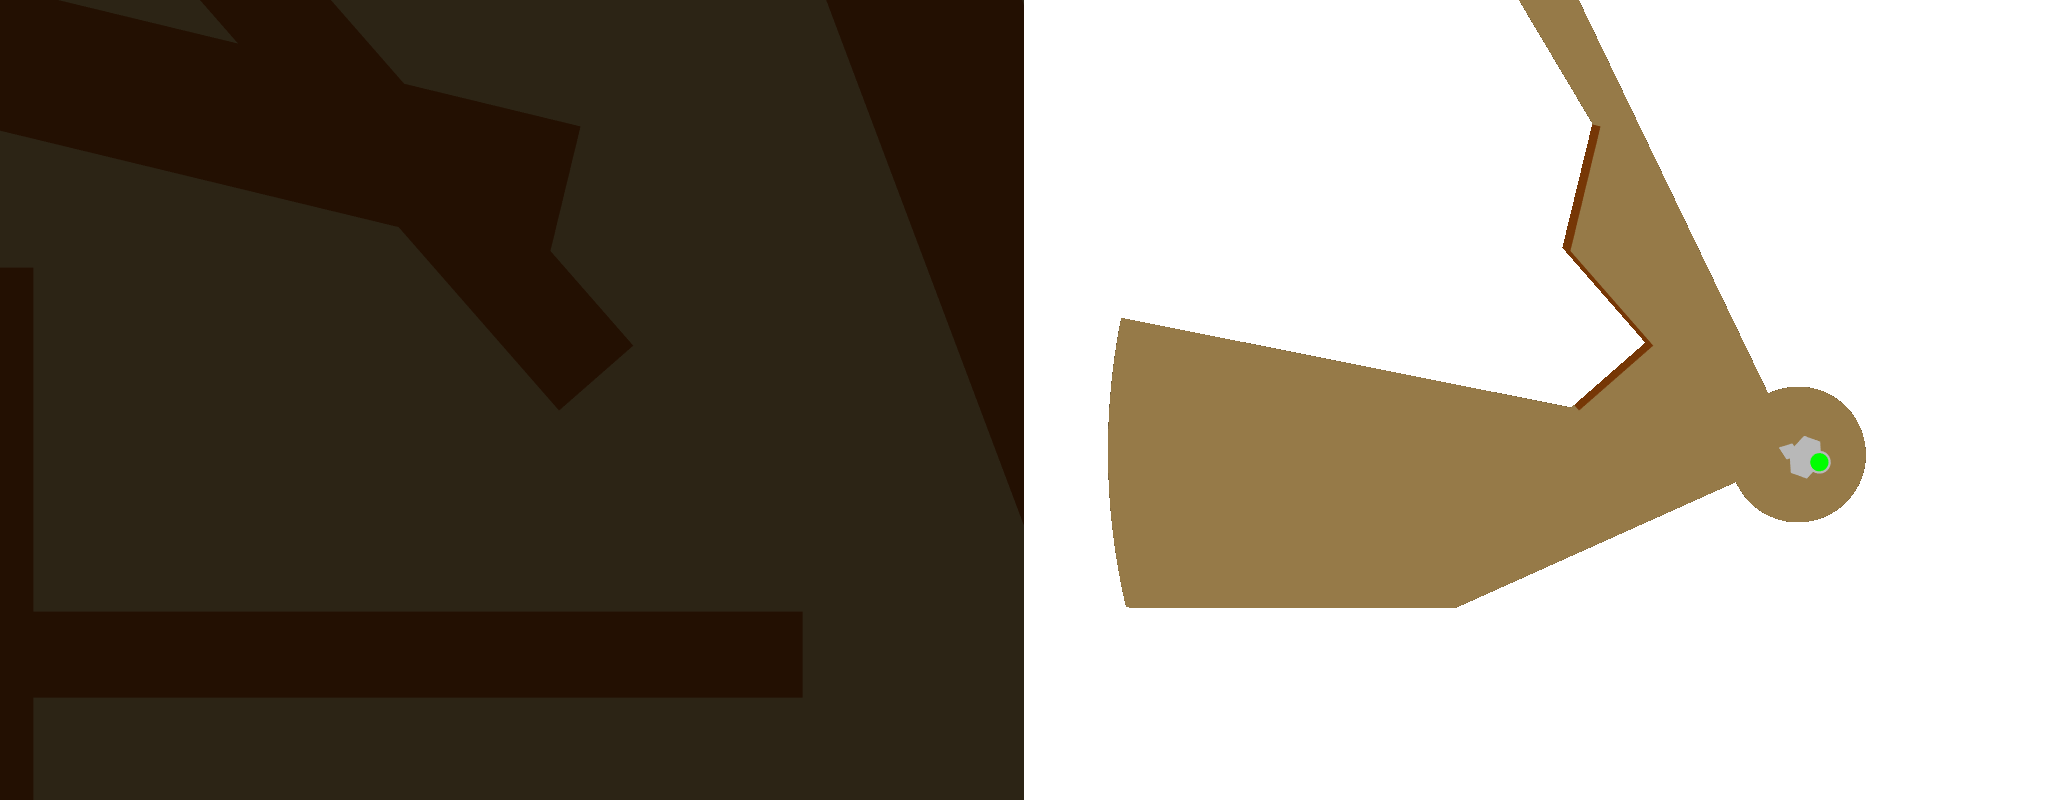
\includegraphics[width=.8\textwidth]{images/CameraRenders}
  \caption[Rendered image from the two cameras]{Showing the fog camera render on the left, and the player camera render on the right.}
  \label{fig:cameraRenders}
\end{figure}

\section{Responsive user experience}
When working on a networked game, providing a responsive user experience for clients is important in the wake of less than optimal network connections~\cite{bernier2001latency}. This section will provide a brief overview on how networking in \emph{Dockit League} is handled to take local responsiveness into account. 

\emph{Dockit League} performs any important calculations like collision checks, damage calculations and cooldowns on the server before synchronizing all of the clients. This is primarily handled through the use of \emph{Command} and \emph{ServerCallback} attributes to make sure certain blocks of code only run on the server before synchronzing through the use of \emph{ClientRpc} functions. \emph{ServerCallback} attributes are particularly useful for when the developer wants collision callbacks like \emph{OnTriggerEnter} or \emph{OnTriggerStay} to only execute on the server. The attribute is only available for \emph{NetworkBehaviour}'s although some workarounds can be made to allow for simiar functionality within standard \emph{MonoBehaviour}'s as mentioned in Section~\ref{sec:networkLimitations}.  

Visual effects on the other hand are handled locally on the clients through the use of synchronized callbacks while client prediction in terms of movement is handled using the interpolation functionality of Unity's \emph{Rigidbody} component.  

\subsection{Consistent force for server and clients}
\label{sec:conForce}
A rather common component to work with in Unity is the \emph{Rigidbody}. These are used for any physics based movement and are generally something the developer would like to keep synchronized across the network. Rigidbodies are synchronized by the \emph{NetworkTransform} component and while one might believe that applying force to the rigidbodies in this case would keep them consistently synchronized across the network, this is actually not the case. In the case of trying to apply force from the player's position towards a point, the server player will experience a stronger amount of force than the clients will. In the case of a peer to peer based game like \emph{Dockit League}, this is unwanted behaviour as the server and clients should experience the same or very similar forces.

We tried a couple of different workarounds like synchronising the code for adding force through the use of \emph{ClientRpc}'s or increasing the synchronization rate of the rigidbodies, but none of these ended up being a usable solution. The issue in general is a result of calculating force vectors on the server based on player positions. This does not necessarily work as by the time the code executes on the clients, their new and updated positions have changed enough to make the force direction different. We ended up trying to use \emph{TargetRpc}'s as a workaround and send the strength of the force, the force mode and the position we wanted to add force towards as parameters. Using this approach allowed the player to locally calculate the force vector and provided far more consistent results than any previous approaches. This also means that the player with authority gets to add the force, as they override the force added on the server. 

\section{Unity's networking limitations}
\label{sec:networkLimitations}
When developing a networked game in Unity, there were a few cases where we wished that the network interface of Unity allowed for certain types of functionality that would make implementation of various features easier. There are a couple of inherent limitations with Unity's current networking capabilities. These include:
\begin{itemize}
    \item \emph{Command}'s, \emph{ClientRPC}'s and \emph{TargetRPC}'s:
    \begin{enumerate}
        \item Are unable to return any data. All functions using these attributes need to return \emph{void}.
        \item Are unable to take component references as parameters. This means that for example sending the \emph{Transform} component of a player is impossible. 
        \item Cannot be overloaded. A separate function with a different name is necessary if different parameters need to be passed. 
        \item Does not support generic parameters. 
    \end{enumerate}
    
    \item Calling any \emph{Command}s requires authority. This is something only the player object has, meaning that any child objects of the player are unable to call \emph{Command}s by themselves. 
    
    \item Standard Unity callbacks will run on all clients by default. This means that any collision callbacks also run on all clients. Unity provides tools for managing this with classes deriving from \emph{NetworkBehaviour}, but not \emph{MonoBehaviour}. 
\end{itemize}

This section will take a look at how some of these limitations can be worked around. 

\subsection{Network spawned objects}
The inability to return data from \emph{Commands} meant that we were unable to acquire references to any game object that the players spawned. A workaround for this problem can be implemented through the use of \emph{TargetRPC} functions which make it possible to selectively run code on a single client. 

In our case, whenever we needed an ability to acquire references back to their spawned game object, we used a combination of interfaces and \emph{TargetRPC} functions in \emph{Docking} to send a reference to the player who spawned the object. This is handled by letting an ability implement the \emph{ISpawnableReferenceProvider} interface and acquire the reference in the implemented function \emph{SetSpawnedObjectReference(GameObject spawnedObject)}. 

Spawning objects is handled through the use of a custom spawning function in \emph{Docking}. This function then looks for the interface and sends a reference of the newly spawned object, as seen in Listing~\ref{listing:cmdSpawnedReference}.

\begin{listing}[htb]
\begin{minted}[fontsize=\footnotesize]{csharp}
[Command]
public void CmdSpawnObjectReference(int abilityId, 
                                    int prefabId, 
                                    Vector3 position, 
                                    Vector3 rotation) {
    
    ISpawnableReferenceProvider ability = dockingKit.abilities[abilityId] 
                                            as ISpawnableReferenceProvider;
    if(ability != null) {
        SpawnableObject spawnObject = SpawnableFactory
                                        .Instance
                                        .SpawnObject(ability.GetSpawnablePrefab(prefabId), 
                                                     position, 
                                                     rotation, 
                                                     netId.Value, 
                                                     player.GetPlayerTeamId());
        
        TargetSetSpawnObjectReference(GetConnectionToClient(), 
                                      spawnObject.gameObject, 
                                      abilityId);
    }
}

[TargetRpc]
public void TargetSetSpawnObjectReference(NetworkConnection connection, 
                                          GameObject spawnedObject, 
                                          int abilityId) {
    
    ISpawnableReferenceProvider ability = dockingKit.abilities[abilityId] 
                                            as ISpawnableReferenceProvider;
    if(ability != null) {
        ability.SetSpawnedObjectReference(spawnedObject);
    }
}
\end{minted}
\caption[Spawning game objects and passing the reference back to the owner]{Code snippet for spawning game objects and providing a reference back to the owner}
\label{listing:cmdSpawnedReference}
\end{listing}

\subsection{Network functionality for MonoBehaviours}
Deriving from the \emph{NetworkBehaviour} class requires that the game object a script is attached to has the \emph{NetworkIdentity} component. The \emph{NetworkIdentity} component automatically handles disabling and enabling of objects during the life cycle of a hosted game. There are cases where the developer might want to manually control this by using \emph{MonoBehaviour} instead of \emph{NetworkBehaviour}, as discussed in Section~\ref{sec:docking}. 

In our case, we let the \emph{Ability} base class stay as a \emph{MonoBehaviour}. In order to provide network functionality for the abilities, we added a reference to \emph{Docking} in the base class as a proxy for networking. This means that any abilities can go through \emph{Docking} to call \emph{Command} functions. The \emph{Ability} base class also includes a variety of virtual callbacks that in turn are called by \emph{Docking}.  This allows abilities to execute synchronized code by overriding the virtual callbacks. 

\subsection{Unity callbacks}
Unity offers several different callbacks that helps the developer manage the life cycle of a script or for collision handling. When working with networked code there are times where the developer wants code to only run on the server or the clients, local or remote. This is easy to do for \emph{NetworkBehaviour} derived classes as they, for example, can use the \emph{ServerCallback} attribute to tell Unity that the attached function only should run on the server. This is of course not possible for \emph{MonoBehaviour} classes although the workaround for this is fairly simple. 

In the case of wanting to make sure that a collision callback for an ability only gets executed on the server, we check for \emph{docking.isServer} at the start of the callback. The \emph{isServer} boolean is part of \emph{NetworkBehaviour}'s and is true if the current code is running on the server. The only issue with this approach is that the callback itself will still get called on all clients, creating some unnecessary overhead even if the body of the function only is executed on the server. We do not see this as a particularly large issue given that collision callbacks won't happen frequently enough for this to be a performance problem.

\section{Programmatic interpolations}
\label{sec:boomerangCurve}
Unity as a game engine already has fairly robust and powerful animation tools that allows the developer to create and manage animations directly in the editor. These animation tools have a lot of versatility, but there are times where the developer might want a bit of extra control and use a programmatic interpolation instead. 

In our case we needed to produce a curve for a boomerang to travel through while developing the boomerang kit. We decided to perform this interpolation through the use of a \emph{Cubic Bezier curve} as these curves are flexible, very simple to control and can provide a nice squeezed arc for the boomerang to interpolate through. Another option would be to use a Hermite curve, but we ended up sticking with Bezier curves as it would make the code more readable for all group members due to everyone's preexisting familiarity with these. The formula for interpolating through cubic Bezier curves is as follows:
$$
B(t) = (1 - t)^3 P0 + 3(1 - t)^2 t * P1 + 3(1 - t)t^2 * P2 + t^3 P3 
$$
The function takes five parameters:
\begin{description}
    \item[P0:] The start position of the curve
    \item[P1:] The handle of the start position
    \item[P2:] The handle of the end position
    \item[P3:] The end position of the curve
    \item[t:]  The input time of the interpolation. Has to be in range [0, 1]
\end{description}

We use the Bezier curve in two ways:
\begin{enumerate}
    \item To create vertices for a \emph{LineRenderer} component that displays the approximate travel path of the boomerang while holding down the ability button
    \item To interpolate the boomerang itself as the ability button is released
\end{enumerate}
When we say approximate path we mean the path that the boomerang would travel if the player stood perfectly still.
The point of displaying an approximate path is to give the player an idea of how far the boomerang will travel before returning. It is generated using local coordinates rather than world coordinates. On the other hand, actually throwing the boomerang stores the world position of both handles while using current position of the player as start and end point. This means that the Bezier curve will dynamically change based on how the player is moving, but still travel to the peak of the approximate path.  

While the Bezier curve is nice for providing a curve to interpolate through, the animation itself looked fairly uninteresting as the change in \textbf{\textit{t}} was linear due to the fact that we simply used a timer variable for it. The boomerang kit's abilities are built around the position of the boomerang so we needed to provide ample time for the player to use the kit's abilities as the boomerang approached the peak of its curve. 

\subsection{Handling the velocity of the animation}
While developing, we drew several graphs that could represent a non linear change in our input parameter \textbf{\textit{t}}, but were unsure of how we could get representations of these into our code. This section includes two different ways of providing graphs that can be evaluated by the game to control the velocity of the animation.

The first solution we found by looking at Unity's documentation was to use Unity's built in \emph{AnimationCurve}~\cite{unityDocumentationAnimationCurve} type. \emph{AnimationCurve}s can be public members of any \emph{MonoBehaviour} class, allowing the developer to use the inspector to generate curves in the range of [0, 1] for both axes by default. These curves also have an evaluation function that allows the developer to provide a input time parameter and get an output back. 

In our case, we wanted the boomerang to accelerate from the start, decelerate towards the halfway point of the animation and then accelerate again towards the end. This was fairly simple to implement using the \emph{AnimationCurve} type since it works in the range of [0, 1] by default. All we needed to do was to provide the evaluation function a time variable and use its output as \textbf{\textit{t}} into the Bezier curve interpolation. 
    
\begin{figure}[tbph]  %t top, b bottom, p page | you can also use h to try to get the figure to appear at the current location
  \centering
  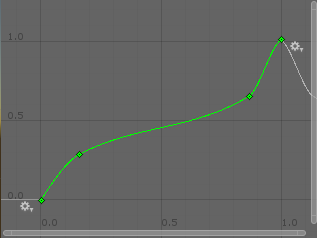
\includegraphics[width=.75\textwidth]{images/BoomerangAnimationCurve}
  \caption[Boomerang animation curve using Unity's built in type]{This curve shows the change in \textbf{\textit{t}} as time goes from 0 to 1 on the x axis using Unity's \emph{AnimationCurve} type.}
  \label{fig:boomerangcurve0}
\end{figure}

\begin{figure}[tbph]
    \centering
    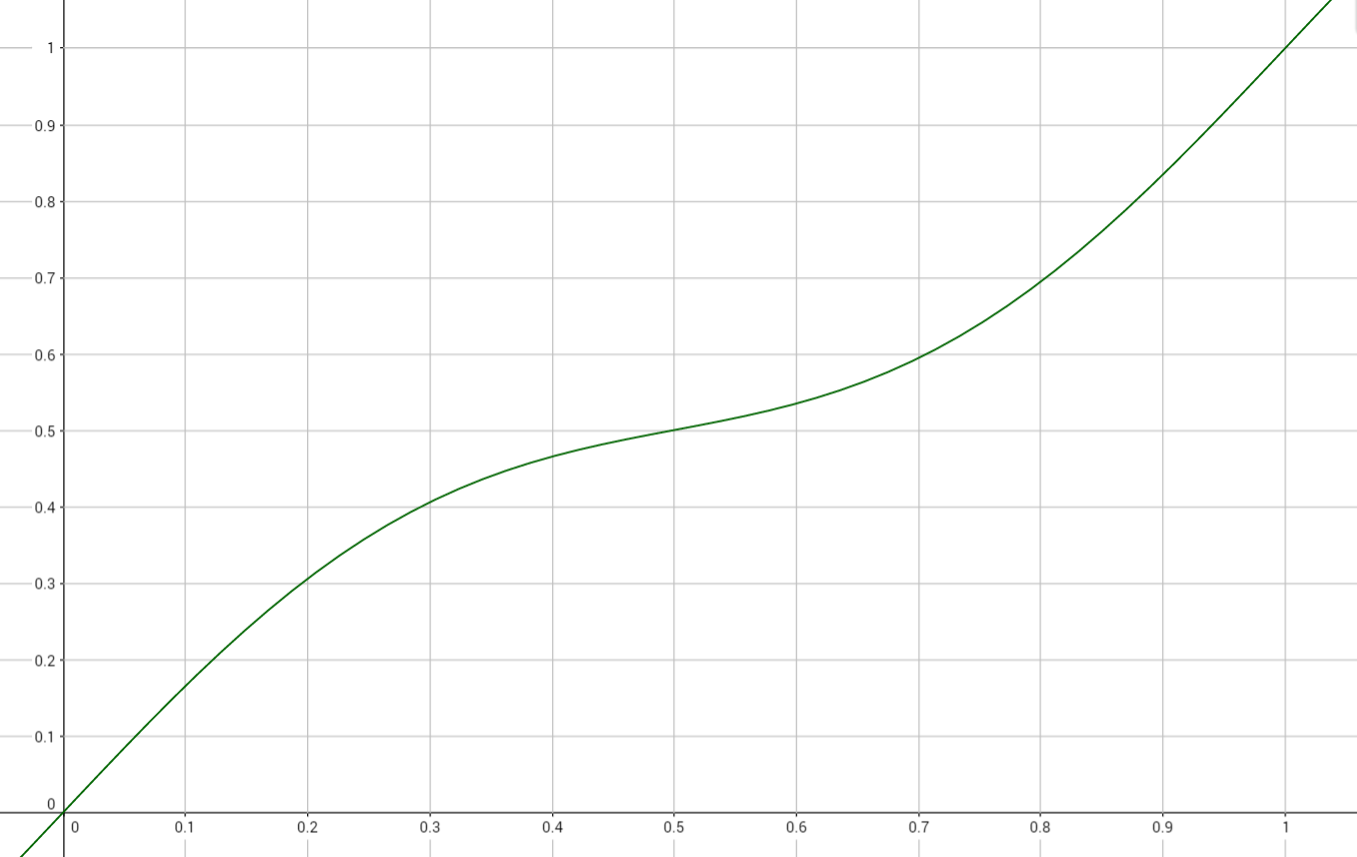
\includegraphics[width=.75\textwidth]{images/BoomerangMathematicalCurve}
    \caption[Boomerang curve using a mathematical formula]{This curve shows the change in \textbf{\textit{t}} as time goes from 0 to 1 on the x axis using the mathematical curve $f(x) = x + sin(6.28x) / 9$}
    \label{fig:boomerangcurve1}
\end{figure}
    
As seen in Figure~\ref{fig:boomerangcurve0}, the \emph{AnimationCurve} approach provides an interface with control points and control point handles which is fairly easy to use, but there is also another way of solving the problem. 

A more generic approach would be to use a mathematical function like $f(x) = x + sin(x) / c$ to create a similar looking curve, but this approach has some problems that need to be dealt with. First of all, the curve needs to be scaled so that the wanted part of it is within the range of [0, 1] for both axes in order for the output to work with the interpolation function. This could be achieved by playing around with a graph plotting tool like \emph{GeoGebra} or similar. In our case, the function $f(x) = x + sin(6.28x) / 9$ as seen in Figure~\ref{fig:boomerangcurve1} would provide similar behaviour to Figure~\ref{fig:boomerangcurve0}, but still lack the strong acceleration towards the end of the interpolation. This approach gives less control to the developers who work in the engine and spending time trying to scale the curves can be quite time consuming.

We also made sure to check the performance difference between the two approaches by measuring the execution time of both. We measured the time spent on each function per update and calculated the mean of the time values after 10 boomerang throws. This gave us the following results:

\begin{itemize}
    \item The average execution time of the \emph{AnimationCurve}'s evaluation function took \textasciitilde$ 0.36 \mu s$
    \item The average execution time of the math function took \textasciitilde$ 0.20 \mu s$.
\end{itemize}

The time difference was calculated using Unity's \emph{Time.realTimeSinceStartup} variable. The \emph{Time.realTimeSinceStartup} float is measured in seconds so we multiplied the average time difference by $10^6$ and used a output precision of two decimals for these results. 
The mathematical approach provides a small increase in performance as seen from the results, but in our case the difference is too small to warrant using it. The \emph{AnimationCurve} approach is far easier to work with directly in the editor instead of using external graph tools to modify the curve to our needs. On the contrary, the mathematical approach is more generic and might see use in non Unity applications.

\section{Interpolation using coroutines}
Interpolations in Unity are generally handled in each script's \emph{Update()} function through the use of timer variables and adding Time.deltaTime to these per update. In some cases this adds unnecessary logic to the update loop of a component and the developer might wish to further decouple the interpolation from the loop itself to improve code readability. This can be handled using C\# coroutines as these functions are capable of stopping execution during a frame and then resuming the next frame to provide similar functionality to that of the standard Unity update loop callback. 

An example of how this is implemented can be seen in Listing~\ref{listing:radiusLerp1} which contains a snippet from the \emph{FieldOfView} component and includes a coroutine for interpolating the view radius of the component.

\begin{listing}[htb]
\begin{minted}[fontsize=\footnotesize]{csharp}
public float viewRadius;

private IEnumerator ViewRadiusLerp(float targetRadius, float speed) {
    while (Mathf.Abs(targetRadius - viewRadius) > 0.1f) {
        viewRadius = Mathf.Lerp(viewRadius, targetRadius, speed * Time.deltaTime);
        yield return null;
    }

    viewRadius = targetRadius;
}
\end{minted}
\caption[Coroutine for field of view radius interpolation]{A coroutine used for interpolation of the field of view radius}
\label{listing:radiusLerp1}
\end{listing}

This function will stop at the end of each while loop execution and resume on the next frame using \emph{yield return null;}. This allows the interpolation to move forwards each frame although the example function in particular will not provide fully linear interpolation. This is due to fluctuations in deltaTime between frames and the observed behaviour of an interpolation using this function will appear as a smooth interpolation that slows down towards its end. A different way of implementing the interpolation, this time in an actually linear fashion would be to use a local timer variable that moves in the range of [0, 1] by adding Time.deltaTime each frame. A modified version of the radius interpolation using this thought process can be seen in Listing~\ref{listing:radiusLerp2}. 

\begin{listing}[htb]
\begin{minted}[fontsize=\footnotesize]{csharp}
public float viewRadius;

private IEnumerator ViewRadiusLerp(float targetRadius, float speed) {
    float lerpTimer = 0;
    while (lerpTimer <= 1f) {
        lerpTimer += Time.deltaTime * speed;
        viewRadius = Mathf.Lerp(viewRadius, targetRadius, lerpTimer);
        yield return null;
    }

    viewRadius = targetRadius;
}
\end{minted}
\caption[Modified coroutine for linear field of view radius interpolation]{A modified coroutine used for linear interpolation of the field of view radius}
\label{listing:radiusLerp2}
\end{listing}

A benefit of decoupling interpolations from the update loop is that there is no need for an additional conditional variable that checks whether an interpolation is active per frame. When reading the code, the interpolation approach also makes it more clear when the interpolation starts using the \emph{StartCoroutine()} function. 
An apparent thought when working with coroutines and interpolation is the possibility of providing a generic solution for all basic interpolations by using of a static utility class. This will not work as Unity requires that all coroutines need to exist in classes deriving from \emph{MonoBehaviour} which is incapable of being static. This can be worked around by having a singleton \emph{MonoBehaviour} class and call functions through its static instance. 

\section{Initial game balancing}
The full game functionality required for proper user testing ended up being implemented rather late into the project's development. Due to this we had limited time for user testing and needed to provide the testers with a build that already had some initial balancing done. 
\emph{Dockit League} is an asymmetrical game due to the variety of available docking kits so we used a mathematical model~\cite{schell2014art} for the initial balance iteration. Doing so allowed us to have a overview over the different kits including their strengths and weaknesses.

\begin{table}[tbph]
\centering
\caption{Initial balance table}
\label{tab:initBalance}
\begin{tabular}{@{}llllll@{}}
\toprule
\textbf{Docking Kit} & \textbf{Health} & \textbf{Movement Speed} & \textbf{Damage} & \textbf{Utility} & \textbf{Totals} \\ \midrule
Boomerang Kit        & Low (1)         & High (3)                & High (3)        & Medium (2)       & 9               \\
Brawler Kit          & High (3)        & Low (1)                 & Medium (2)      & Medium (2)       & 8               \\
Bomber Kit           & Medium (2)      & Low (1)                 & High (3)        & Medium (2)       & 8               \\
Marksman Kit         & Medium (2)      & Medium (2)              & Medium (2)      & Medium (2)       & 8               \\
Sniper Kit           & Medium (2)      & Medium (2)              & High (3)        & Medium (2)       & 9               \\
Tank Kit             & High (3)        & Low (1)                 & Low (1)         & High (3)         & 8               \\
Trapper Kit          & Low  (1)        & Medium (1)              & Medium (2)      & High (3)         & 8               \\
Support Kit          & Medium (2)      & Medium (2)              & Low (1)         & High (3)         & 8               \\ \bottomrule
\end{tabular}
\end{table}

Balance Table~\ref{tab:initBalance} contains columns for kit name, kit health, kit movement speed, damage and utility. The damage column has values assigned based on the potential damage output of the kit while the utility column has values assigned based on the overall the utility the kit provides through its abilities. This includes abilities that apply modifiers and other effects without necessarily focusing on damage. Further tweaking on cooldowns, damage values and modifier durations is the focus of the user testing rather than the initial balancing as this Section is supposed to give a rough estimate of each kit's capabilities. 
Additional information on the various docking kits and their abilities can be found in Section~\ref{sec:dockingKits}

\subsection{Observations from the initial balance table}     
As seen in Table~\ref{tab:initBalance}, the sniper and boomerang kits end up with a slightly higher total than the other kits. This is a deliberate decision as both kits have a high damage potential if played well, while having a low to medium damage potential otherwise. We believe that both kits are fairly challenging to play in order to achieve their full damage potential, so the difficulty offsets the fact that the two kits are a bit stronger than the rest. 
The boomerang kit requires the player to hit with multiple boomerangs while they move forwards and then again once they move back for the maximum amount of damage. The sniper kit requires time and preparation before shooting and rewards a large amount of damage if the projectile actually connects.  
These aspects of the two kits allows us to provide a high risk, high reward ratio for playing well.

An interesting thing to note with our current design is that none of the implemented kits have a low utility value. All the kits feature at least two abilities that provide utility through either the use of modifiers or other effects. The utility abilities for the kits are generally designed to help patch up the weaknesses of each kit. The brawler kit, for example, struggles fighting ranged enemies due to its low speed and melee weapon, but contains abilities for reflecting projectiles and stunning opponents to get closer. If any future development were to take place on the project, creating kits with less utility and a larger focus on the other statistics could improve the variety of of the kits.

One important aspect of game balance is the fact that distinct weaknesses is a great way to provide counterplay and avoiding dominant strategies~\cite{gameBalanceWeaknesses}. While the kits generally have abilities that help them somewhat with their weaknesses, these abilities have long enough cooldowns to not always be available. Balancing cooldowns isn't the only way to expose the weaknesses of kits though. 
The boomerang kit is the only kit with low health and has a large damage potential with high movement speed. One of the weaknesses of the boomerang kit is the low health, and being caught unaware by enemy players will lead to a swift death. The limited field of view also helps creating situations where the player might have been inattentive and not seen an enemy sneaking in from behind. The high speed of the kit might be seen as beneficial, but can result in the player carelessly rushing into enemies who are right around the corner of walls and other obstacles. 

Another thing to note about the balance table, is that it does not take shop price into account. This is due to the fact that we were unsure of how strong each kit was before performing playtesting, so we kept the same price for all docking kits. Starting to think of price as part of the initial balance table would allow for certain kits to be stronger than others by justifying their strength with a higher price. Given a larger pool of docking kits fulfilling similar roles than currently implemented in the game, the price could end up being used to a larger extent to create more variety for kits with similar use cases. 
 
\section{Controller based menu navigation in Unity}
\emph{Dockit League} originally had a different main menu and lobby handling script that was more integrated for controllers, but we ended up having to cut it from the last iteration of the game as there was limited time to integrate it with the new lobby and main menu that supported different game modes. We would like to spend some time detailing the old implementation in this section as it might provide additional insight into how controller based menu navigation can be handled in Unity. 

There are two primary things that should be handled differently to accommodate for controller navigation compared to just navigating with the mouse:
\begin{enumerate}
    \item The controller needs an entry point for navigation compared to the mouse. These usually consist of clickable buttons and can be navigated through using the dpad or left analog stick of the controller. 
    \item While having a back button on menu screens is common for mouse and touch navigation, controller users might find it more intuitive to be able and navigate backwards using a physical button. One needs only look back at the era of the \emph{Super Nintendo Entertainment System} and its games to see that developers already were using a physical button for backwards menu navigation. 
\end{enumerate}

Backwards menu navigation can be handled in multiple ways. The current implementation in \emph{Dockit League} allows for arbitrary menu navigation and works well with mice, while the old implementation used a stack instead, inspired by how \emph{Android} handles backwards navigation using its fragment back stack~\cite{androidBackStack}. 

The stack based approach allows for simple controls when using the \emph{OnClick} interface to handle individual button presses. The developer simply has to drag the next menu object as a parameter to the menu handling script and the script then takes care of putting the old menu panel into the stack. Once the new menu panel had been displayed the script would quickly look for buttons and set the first found button as the selected one, providing an automated entry point for controller navigation. 

This old implementation also supported adding properties to the top of the stack, allowing custom behaviour on backwards navigation. We handled this by storing enums with the menu stack objects and perform custom behaviour depending on the enum of the popped menu. This was particularly useful for telling Unity to stop hosting or matchmaking whenever the player left certain types of menus. 
The stack based approach also made it easy to use physical buttons for backwards navigation as all the script needed to do was to wait for the correct button to be pressed and then trigger a backwards navigation by popping the stack. 
\chapter{Deployment}
\label{chap:deployment}

\section{Automated Unity Builds}
While Unity and Git don't necessarily work too well together out of the box as mentioned in Section~\ref{sec:unityGit} one might start to wonder whether automatic build processing is possible. Having a central hub with automatically built binaries can be quite useful for testing the game and providing the correct binaries for testers. Unity offers a free service called \emph{Unity Cloud Build} which provides this functionality. 

\begin{figure}[tbph]  %t top, b bottom, p page | you can also use h to try to get the figure to appear at the current location
  \centering
  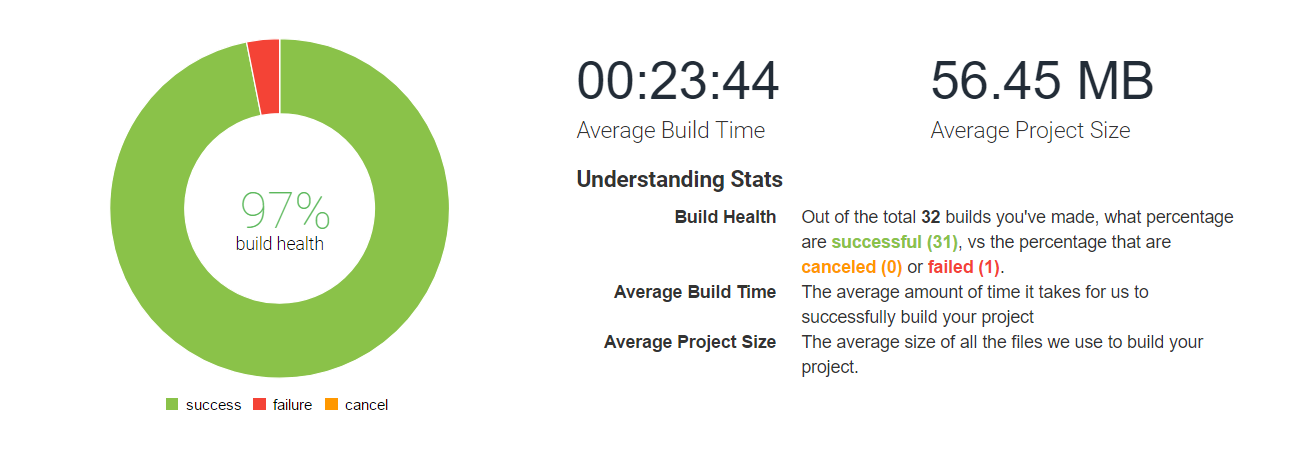
\includegraphics[width=\textwidth]{images/unityCloudBuildStats}
  \caption[Project statistics from Unity Cloud Build]{Unity Cloud Build's project statistics illustrate the status of the build process.}
  \label{fig:unityCloudStats}
\end{figure}

Unity Cloud Build allows the developer to set up automatic builds for different target platforms and integrates with BitBucket using SSH keys to get access to the project repository. Specific branches to be built can be specified directly within the service and provides shareable links which can be given to others for both deployment and testing purposes. The service also offers build statistics as seen in Figure~\ref{fig:unityCloudStats} and allows for automatic execution of specific unit tests. 

We have integrated our BitBucket repository with Unity Cloud Build to make sure that we always have an up to date build available for Windows, MacOS and Linux. 

\subsection{Dockit League binaries}
This section contains the binaries for the game which are built at the time of thesis hand in through the use of Unity Cloud Build's shared links. In order to download the latest build of \emph{Dockit League} we recommend visiting the BitBucket repository~\cite{bitbucketRepo} and download the binaries from the links on the front page. There is no necessary installation needed when downloading the game as the downloaded folder includes all the files for the game. 

These are the links to the different builds:
\begin{itemize}
    \item Windows x86:  \cite{x86build}
    \item Windows x64:  \cite{x64build}
    \item macOS:  \cite{macOSbuild}
    \item Linux:  \cite{linuxbuild}
\end{itemize}
\chapter{Testing and User Feedback}
\label{chap:testing}
If you are developing software you must do some testing with users.  This chapter describes those tests and what you learnt from the tests.  This should include the selections of questions that you were intending to answer when you started the test.  

\todo{ In house testing, per implemented feature, per review meeting }
\todo{ Actual testing with other users }
\chapter{Discussion}
\label{chap:discussion}

\section{Development decisions}
\subsection{Using scriptable objects}
\label{sec:scriptableObjects}
When we first started working on the modifier architecture for Dockit League, we had to find an easy to use and extendable way of creating new modifiers. Having recently seen a talk from \emph{Unity Europe 2016}~\cite{scriptableObjectsTalk} about how scriptable objects can be used for these types of use cases, we decided to base the architecture around them. Using scriptable objects instead of \emph{MonoBehaviour} has a wide range of advantages:
\begin{itemize}
    \item A scriptable object is not reset when exiting play mode compared to a \emph{MonoBehaviour} object. This means that any values tweaked in the inspector while playing stay saved.
    \item Scriptable objects can be referenced instead of copied when instantiated, helping decrease unwanted redundancy for complex objects. 
    \item A scriptable object can be referenced from any scene while keeping cross-scene references of \emph{MonoBehaviour} objects can be tricky. 
    \item Scriptable objects provide better version control granularity as one file gives one object without anything additional like transform components. 
\end{itemize}

Scriptable objects also have some disadvantages:
\begin{itemize}
    \item Scriptable objects have very few callbacks compared to a \emph{MonoBehaviour} object. \emph{OnEnable()}, \emph{OnDisable()} and \emph{OnDestroy()} are the only ones. This can be worked around by having a proxy \emph{MonoBehaviour} that calls functions within the scriptable object. 
    \item Scriptable objects contain shared data. This means that any object references during runtime only should be acquired and used in method scope. 
\end{itemize}

In the case of our project. Using scriptable objects for modifiers and shop items gives us the ability to create and quickly edit data directly in the editor as well as being able to attach some additional code if necessary. 
In the case of modifiers, using scriptable objects makes it very easy to define custom behaviour through the use of the multiple callbacks that exist within the base \emph{Modifier} class. These can be overridden to perform code for the server only, on all clients and locally which gives us the amount of control we want when working on a networked multiplayer game. 
In the case of shop items, using scriptable objects provides a reusable interface that allows us to quickly add items without having to worry about editing other dependent components as the shop itself handles instantiation and placement of these.  

A more technical look at how scriptable objects are used for modifiers and shop items can be found in Section~\ref{sec:modifiers} and Section~\ref{sec:scriptableObjectsShop}.
    
\subsection{Moving from Confluence to ShareLaTeX for writing the thesis}
As seen in Appendix~\ref{app:projectPlan} we had originally planned to use Confluence as the thesis container as that would mean having a centralized hub for documentation and the thesis. We eventually started moving away from Confluence and ended up only using it to document any Scrum related meetings and started using ShareLaTeX instead. The reason for this is that it allows the thesis to look more professional due to the template style sheet as well as providing a lot of utility tools that make writing the thesis easier. Some of these include easy access to PDF compilation, BibTeX for formatting and automating references as well as being able to work on the thesis in a parallel manner similar to Google Docs. Another benefit of using ShareLaTeX is that less time is spent worrying about text formatting as this is mostly handled by the stylesheet from the thesis template. 

\subsection{Decreasing the amount virtual functions using interfaces}
The \emph{Ability} base class in an important intermediary component for making the docking kits work with networked code. The script itself is not a \emph{NetworkBehaviour} so it instead employs virtual functions that get called by networked components to provide synchronized behaviour. One of the issues we experienced throughout development was the fact that this class would get exceedingly bloated with virtual functions as more features were required. The worst offender were the functions that allowed abilities to have server callbacks, providing similar functionality to the \emph{ClientRpc} attributes of \emph{NetworkBehaviour}'s. The issue here was that whenever we wanted to pass parameters we had to first create a new command in the \emph{Docking} script due to not being able to overload commands or provide generic parameters. We then had to create a corresponding virtual function taking the parameters in the \emph{Ability} class. 

We ended up using interfaces to somewhat alleviate the code bloat. The difference with using interfaces is that we no longer need to create the additional virtual functions in \emph{Ability} for each new type of parameter. Instead, individual abilities can implement the \emph{IServerCallback} interface which supports generic parameters. Using this approach decreases the code bloat a little bit, but we still need to create new commands in \emph{Docking} due to the inherent limitations of commands. In any case it helps reduce a little bit of code bloat so we found it a worthwhile solution. 

\subsection{Providing ergonomic controls when using a twin stick scheme}
\label{sec:ergonomicControls}
During the early design phase one of the things we had to decide on was how many abilities each docking kit would have. We wanted each kit to have enough depth so that players would have to spend some time properly learning each kit and improving their play through experience, but we also had to take into account the control scheme that we were targeting. The abilities of each kit should be easy to access when using a controller while moving about and aiming at the same time. This leaves us with a rather limited selections of buttons to use. 

We have the shoulder buttons, triggers and stick buttons available. We decided that each kit would have four abilities each as the triggers and shoulder buttons are the most ergonomic to use with the dual stick scheme. Using the stick buttons for additional abilities would also have been possible, but we could imagine some imprecise aiming if for example an ability was bound to the right stick button. Less frequently used functionality like opening the shop and docking/undocking could then mapped to the primary ABXY, Start and Select buttons.

\subsection{Updating game engine versions during development}
\label{sec:updatingGameEngine}
Whenever developing games in a constantly updated engine like Unity or Unreal it is inevitable that new versions are released. These new versions come in different shapes and forms. Minor releases mostly contain bug fixes and small changes while major releases introduce new functionality and might end up deprecating old features. In cases where changes or new functionality might be beneficial for the project, one has to see whether spending the time and resources on the upgrade is worth it. 

While testing the game during sprint reviews, one of the issues we ended up experiencing at times were random disconnects with seemingly limited error messaging given for debugging. Researching into the issue a bit on the Unity forums suggested it could be related to the 4KB/s bandwidth limit of Unity. At the same time the issue could simply be related to a inconsistent wireless network at the location we were testing, but we started to think a bit about bandwidth optimization anyways. 

One of the most apparent optimization's we could perform was to move from Unity3D back to Unity2D with the release of Unity 5.6. We originally started working with Unity3D due to the fact that it provided \emph{NavMeshes}~\cite{unityNavMeshes} which would be beneficial in the case that we had the time to work on player bots. Unity 5.6 introduced \emph{NavMeshes} for the (x, y) plane making it possible for us to port the game back to 2D. Doing so would substantially decrease network bandwidth usage since there were no dependencies on 3D components. 

One of the pieces of data we synchronise often are \emph{Vector3}'s consisting of three floating point values. Synchronized \emph{Rigidbody} components in particular consist of many physics related vectors~\cite{unityRigidbody}. Moving to Unity2D would cut the bandwidth usage for any Rigidbody and vector synchronization by $\frac{1}{3}$ which is a fairly significant improvement in network performance. Another side effect of moving over to 2D would be cheaper ray casting. The \emph{FieldOfView} component uses a lot of ray casts to create its view mesh so the performance of this script in particular would improve. 2D Raycasts also give some additional quality of life functionality like providing sorted arrays in order of distance from the origin point when raycasting for multiple colliders.  

Another useful piece of functionality that only works with Unity2D is the \emph{PolygonCollider2D} component which allows Unity to dynamically create colliders out of sprites. Unity offers similar functionality for 3D using the \emph{MeshCollider} component, but creating sprites is generally far quicker and easier than using 3D models for simple shapes like cones and hollow circles. 

We ultimately decided against transferring over to Unity2D due to the fact that the release of Unity 5.6 happened very late into the development cycle. We thought that moving over to Unity2D would take too much time and given that we had no conclusive evidence of hitting the bandwidth limit we would rather spend the resources on writing and improving the thesis instead.  

\subsection{Player field of view versus raycasts for visibility checking}
One idea that we thought of while developing was to use the field of view component for visibility checking rather than regular ray casting. This would allow abilities like the flash grenade in the brawler kit to only stun players who had the grenade in their field of view at the time of explosion rather than using a raycast + dot product. We ultimately decided against implementing this due to a few reasons. 

The first reason is that the field of view is fairly computationally expensive. The component uses many raycasts to dynamically generate a mesh that we use as a visibility mask for the players. It would not be possible to directly synchronise the generated meshes so we would have to synchronise the various variables for the component itself and reconstruct the field of view on the server. Doing so would allow us to have a player local field of view for the sake of responsiveness while using the server's version for any visibility checking. This could work if the server was ran as a dedicated server, but our project is primarily focused on trying to create a MOBA using peer to peer connectivity so a implementation like this would not be very effective as it would place a lot of extra load on the host player. 

A server authoritative visibility check like this would be far better for security reasons compared to local checking. We currently have a middle ground where the server uses raycasts and dot products to check player face directions. This is independent of the field of view component so we have less control in regards to limiting the view angles as the server would need to acquire the view angle of the clients to check consistently with their current field of view.

Another issue is that keeping the field of view synchronized would take a fair share of additional bandwidth if we want the server to keep itself updated frequently. Given the fact that players move and are able to rotate quickly and arbitrarily, a very high update rate or interpolation would have to be employed for the server to stay consistent with the local player. Since players can rotate arbitrarily and quickly, using interpolation for the field of view would be somewhat of a challenge as determining whether the player rotated clockwise or counter clockwise to the current rotation would be hard without synchronising additional data. This would require a fairly massive rework of the current implementation.  

\subsection{Sticking with dual stick controls}
Dockit League is primarily developed with a twin stick controller setup in mind. This is mostly due to the fact that other control options were outside of the scope for the project. One might think that providing similar controls through the use of a mouse would be simple, but it brings somewhat of a balancing issue. 
Making the player face towards the direction of the mouse pointer is generally what we would think of as the simplest and most intuitive implementation of the mouse control scheme. The main problem with this implementation is that aiming becomes easier for players using a mouse. To give an example, two players standing still at different positions want to fire at each other with a projectile. One uses a mouse while the other uses a controller. The player using the mouse can simply hover the mouse cursor over the other player for accurate aim while the player using the controller needs to aim by approximately pointing the right stick in the correct direction.  

To provide similar behaviour between the controller and mouse options we would need to make the mouse controls work more similarly to that of a controller stick. The mouse cursor could be hidden and reset to the center of the screen each frame while recording any changes in mouse movement as a direction vector. This vector could then be used to make the player point in the same direction that the mouse is moving. This would balance the two control schemes to some degree, but we believe that mouse controls like the ones we described might end up feeling too unintuitive for players. Due to this we ended up deciding to stick with the controller dual stick scheme for our project scope. 
    
\section{Experiences with the HLAPI of Unity}
The HLAPI of Unity has been very useful for us when developing \emph{Dockit League}. It provides a good high level API that has somewhat of a learning curve, but is generally easy to use once we had worked more with it. It is not without its flaws however. Certain functionality like host migration is still broken to this date as noted by other developers on the Unity forums~\cite{forumsUnityNetworkFeedback} and Reddit~\cite{redditUnityNetwork}. Host migration in particular is a very essential feature for a peer to peer based game as it prevents everyone from disconnecting when the host disconnects. There is also somewhat lacking debugging tools available for the networking. A lot of error messages related to disconnects are vague and it is also not possible to directly measure bandwidth usage in the profiler. This would be useful for developers wanting to know how much of the bandwidth limit they used so they could optimize parts of the networking accordingly. 

The base documentation for Unity's network components is fairly decent in our opinion, but there are parts where the quality of documentation drops to an unacceptable level. The \emph{LobbyManager} and its lobby related systems are horribly documented with only two example projects available in the Asset Store. There is a distinct lack of overarching documentation for how the lobby components work in these projects. To quote the documentation from one of the sample projects on the Asset Store~\cite{unityAssetLobby}: 

\begin{quote}
"The main prefab is in "Prefabs/LobbyManager". This is a canvas with the LobbyManager script on it.
It have multiple child that setup the UI \& different "screens" of the lobby (i.e. Server List, Player Lsit etc...)

Everything above the "Unity UI Lobby" section in the Manager Inspector is from UnityEngine.Networking.NetworkLobbyManager, so see the doc
for it to see an explaination for all of them.

Prematch countdown is the time between all players being ready \& the game starting.

The Lobbymanager script have reference to all the different screens for easy access.
*if you totally replace one of those screens, set its reference there*"
\end{quote}

The documentation in the project is filled with badly written grammar and refers to documentation that barely exists on Unity's web pages. 

\section{Observations from sprint statistics}
\begin{figure}[tbph]
    \centering
    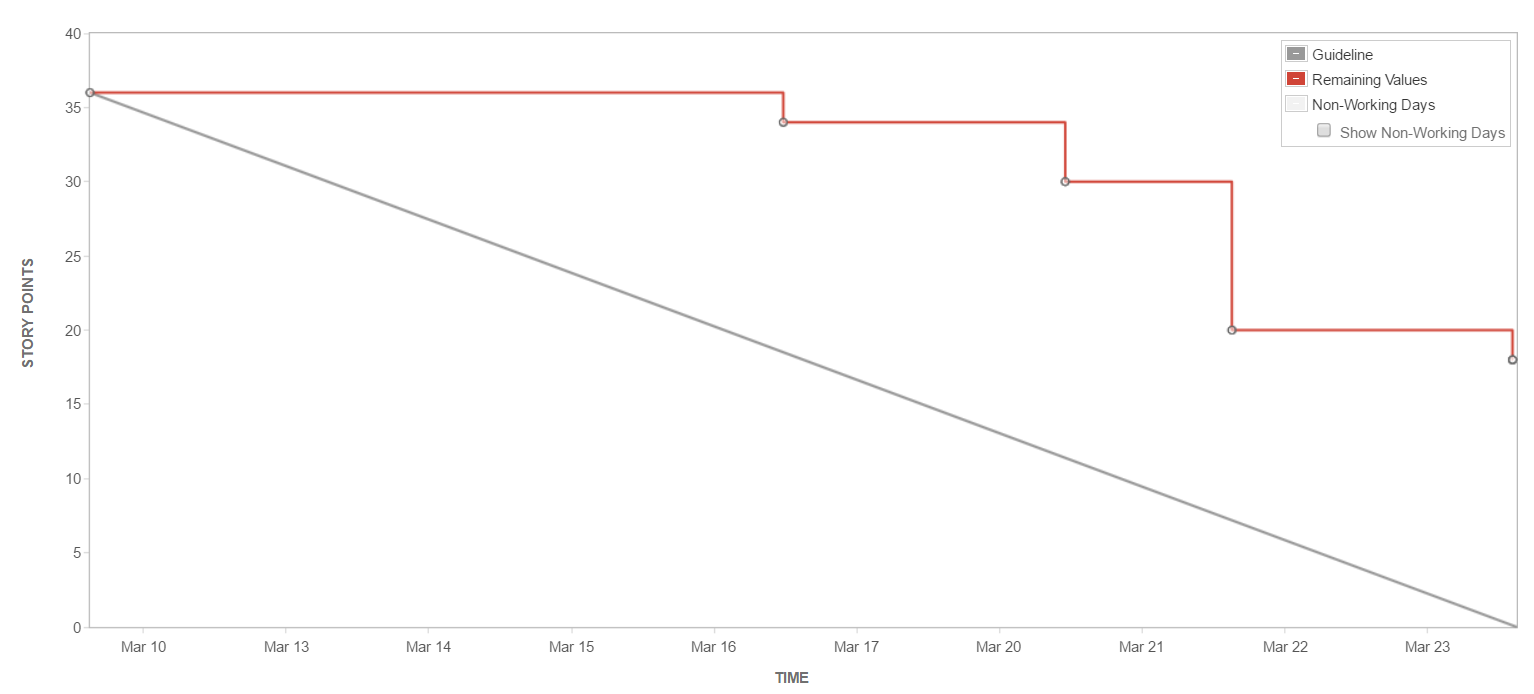
\includegraphics[width=\textwidth]{images/DOCKLSprint4}
    \caption[Burndown chart from the 4th sprint]{The burndown chart for the 4th sprint shows how sprints generally progressed on average throughout the project.}
    \label{fig:burndownChart}
\end{figure}

We will take a brief look at Figure~\ref{fig:burndownChart} which illustrates the burndown chart of the 4th sprint during development as it shows data that was fairly consistent throughout the other sprints. 

The first observation is that most issues generally were finished throughout the second week of the sprint rather than issues regularly finished as the guideline suggests. This is mostly due to the fact that the issues were rather large and not split up into subtasks very often. Doing so would better reflect project progress on Jira, but at the same time this would incur a fair amount of additional overhead per sprint by having to set up subtasks per issue. 

The next apparent observation is overscope. Most of the sprints after sprint 1 ended up having some overscope. The overscope was mostly related to being able to finish a docking kit while also working on other functionality of the game at the same time. This could certainly have been improved by looking at the statistics of previous sprints and manage expectations accordingly. The estimations for some of the game functionalities ended up being estimated for lower story point values than they required due to unexpected issues and bugs which resulted in a lack of resources needed to finish some of the docking kits for the sprint. 

\subsection{Looking at the use of Scrum in retrospect}
In relation to actually working on docking kits, fortnightly sprints ended up fitting well. Designing and implementing the base functionality of most kits required one week of time while the other week was spent on bug fixing and polish. 

Working with Jira allowed us to setup sprints and issues in a tidy manner, but had a lot of additional functionality we never used although we can imagine a lot of it being useful for managing larger teams. 

Despite there having been some overscope during development, using Scrum allowed us to continue developing new increments without necessarily cutting or rushing core functionality of the game due to direct deadlines. The benefit of also having a rather relaxed scope for the game was that it meshed well with Scrum and agile development in general. 

The daily standup meetings in particular were quite useful to us. They helped each group member to stay updated with the different components of the project and worked well as a daily discussion around core functionality requirements as the development progressed. There was a fair amount of uncertainty around the requirements for the core components at the start of the development process. As more kits were implemented we started being able to use these daily meetings to discuss the various requirements our components needed to work with the designs of the different docking kits. 
\chapter{Conclusion}
\label{chap:conclusion}

We are happy with choosing Unity as our engine as we learned a lot of new things in the process of developing the game. We got a better understanding of the HLAPI and its strengths as well as weaknesses. The Unity low level API was also available, but we didn't delve too much into its functionalities. There are currently alternatives to the HLAPI in development~\cite{photonThunder} which could fix some of the issues we experienced and having already used the HLAPI allows us to better judge and compare these API's in the future.

We ended up with a good and flexible architecture in terms of adding new Docking Kits, Abilities and Modifiers as seen from the amount of kits we ended up making. This is also in part thanks to \emph{Scriptable Objects} which we learned to use during development. The knowledge of how to use \emph{Scriptable Objects} is something that will be very useful for any future development in Unity. 

The game might not have gotten as robust networking wise as we might have wanted due to there not being time for much polish, but despite this, we didn't run into any major network related bugs during playtesting so the code and architecture is fairly stable in that regard. We managed to meet our learning goals by implementing a large project with large networked components although there wasn't much time for balancing other than the initial balance iteration. Designing and implementing docking kits with varying and interesting abilities ended up being quite the challenge, but we are very happy with the amount of kits we managed to implement in the end. 

We gained experience with how to use tools like Jira by integrating it with BitBucket and managing issues in the backlog through the use of smart commits. We also found Jira to be a very helpful tool for Scrum activities like planning poker and managing sprints. Confluence was less used than originally intended, but we still attained some further knowledge by using it as a tool for meeting notes and design decision documentation. 

\section{Future Work}
\label{sec:future}
As we mentioned in Section~\ref{sec:feedbackReflect} we will be spending some time before the presentation to polish the game and visuals. We might also end up taking some of the other feedback from the playtesters and tweak various parts of the game while doing the visual polish for a better game experience. Other than that, we have no future plans for the development of the game after the presentation.  



\bibliographystyle{ntnuthesis/ntnubachelorthesis}
\bibliography{inc/BachelorExample}

\appendix %after this line all chapters will have letters instead of numbers
\chapter{Initial Project Plan}
\section{Background}
We’re three game programming students, and naturally we are going to make a game to end our degree as that is what this bachelor is about. We want to use this project to learn valuable skills preparing us for the future. The design of the game allows us to focus on the networking aspects of game development. Figuring out good practices for local responsiveness coupled with consistent networked behaviour and how to implement these is something we would like to learn. This is good knowledge to have in a world where multiplayer, and the ability to stay connected is very important, even in games.
The amount of abilities will challenge us when it comes to game design and balance between a large amount of components, and will push our knowledge in the design aspect of game development. 

\section{Technology}
We’ll use Unity as a game engine. Unity is an engine used by a lot by Norwegian developers, and an engine heavily used worldwide~\cite{unityUsageStatistics}. We already have some experience with Unity, so we want to expand our knowledge. 
Using a game engine is beneficial because it allows us to focus on making a game, rather than constructing the components we need to create a game. 

We will be using Toggl as our primary tool for time tracking. It’s easy to use and allows us to track time spent by the team and what we spent time on. Another benefit of using Toggl is that it can be integrated to Jira allowing us to display time data directly in Jira. 

We will use a combination of Jira, Confluence and Bitbucket for project management and issue tracking, documenting and source code respectively. These are to be part of the professional programming course, and we already have some experience using these tools. They’re all part of Atlassian software development tools, which makes them fairly easy to integrate with each other.

Our primary IDE will be Visual Studio 2015 as it provides us with integrated testing tools with Unity like breakpoints and step by step debugging.  

Group communication will be done through Discord as all the group members are familiar with it and uses it regularly.

\section{Project Goals}
The goals of this project is to have a balanced and entertaining game at the end of semester. In addition to being robust in the sense of proper handling of disconnects, packet delays and packet loss.  During this project we want to learn and improve our Unity knowledge. We want to learn more about networking in Unity, how we effectively handle client/server verification and how we provide a consistent and responsive user experience locally. We also want to improve our knowledge regarding Artificial Intelligence by implementing player-like bots (possibly self-learning) and a “replay highlight selection”-AI if there is enough time. 

One of the other things we want more experience with is asymmetric balancing on a larger scale. We will have to balance individual abilities as well as entire kits. This has to be balanced towards multiple players using different kits in combination with each other. We will have to make sure that overall docking kit balance is somewhat good to avoid scenarios where everyone just uses the same docking kit because it is superior in each and every case. In the Standard Game Mode docking kits will have different prices, and therefore their strength needs to correspond the price.

Although the visuals are not our priority we’ll use Unity shaders for different visual effects, for instance abilities. The fog of war will be solved using masking shaders. We want to learn how to make use of professional tools such as Jira and Confluence for project management. We want to improve our ability to estimate the time it takes to implement features and work with smart/semantic commits for issue management.  

\section{Scope}
\subsection*{Areas of Expertise}
This project will include many disciplines from game development and game programming. The main parts of this will be gameplay design and balancing abilities for docking kits, and then network these. We’ll also need to handle user input, and the responsiveness challenge when it comes to users triggering networked abilities. We’ll have a user interface to display each ability and player health. Graphics and animations will be simplistic and somewhat abstract since this isn’t a priority, and we’re no artists.

\subsection*{Scope Limitations}
We will be focusing on finishing the standard game mode first and add a few docking kits. The scope is variable due to the nature of the game. It focuses on having a variety of abilities, and we can simply add/drop making more as the project goes on. The same goes for game modes.

\subsection*{Task Description}
Dockit League is a top-down multiplayer battle arena game in which players control vehicles that gets different abilities by equipping docking kits. 
Taking inspiration from key features in other popular games, we hope to make a fun and unique experience.

The Standard Game Mode features two teams that play against each other in multiple short rounds, before swapping sides. The sides are asymmetric, meaning if the round timer runs out, the attacking team loses. There will be control points around the map, the attacking team needs to conquer one of these in order to win the round.

Each player can equip one docking kit. These kits consist of four abilities each. In the Standard Game Mode these kits may be bought during the buy time at round start, and the price will vary depending on kit strength. This means that a player will have to save their currency over multiple rounds in order to get any kit.
Most of the abilities have some sort of interaction between each other, both within a docking kit, and with other kits. This allows teams to choose between different strategies, either for executing a strategy themselves, or to counter the enemy's strategy.

The players will have a field of view and a sight radius, the size of these may vary depending on their equipped docking kits. Areas outside of this field will be fog of war. 

\section{Project Structure}
\subsection*{Roles, Responsibilities}
We have divided the group into roles and responsibilities. Martin has been appointed as project lead while Andreas and Sondre are developers. Other responsibilities:
\begin{description}
    \item[Andreas:] Documenting meetings/decisions
    \item[Martin:] Scrum Master
\end{description}

\subsection*{Group rules and routines}
We have outlined some group rules as an attachment to the project agreement. Other than those, some general routines will be to document all design decisions and write short summaries from all meetings in Confluence. All group members are required to show up to meetings. If this is not possible, a notification from the missing group member is needed beforehand.

\section{Planning, supervision and documentation}
\subsection*{Choice of system engineering model}
We have decided to use Scrum for this project. Developing games is generally an agile and iterative process, and being flexible is a must. Therefore an agile model like Scrum is ideal for the project.  Another reason for Scrum is that we wish to learn using professional tools like Jira and Confluence. Scrum works nicely with both of these. Finally, using Scrum allows us to generate a lot of extra documentation during the project due to the amount of meetings, which is going to be quite useful when writing the thesis itself. 

We are planning to have fortnightly sprints with daily standup meetings. Thursdays will be used for “sprint meetings” consisting of the review, retrospective and planning meeting. Each meeting will have a short summary written which will be added to the Confluence pages. 

\subsection*{Plan for status meetings and decision points}
We do not have any external clients for this project, but we will have regular status meetings with Simon McCallum who is the project supervisor. 

\section{Quality Assurance}
\subsection*{Documentation and code standard}
We will be using a good amount of Atlassian’s available tools for the project. Confluence will be used for documentation and as the thesis container while Jira will be used for management of Scrum and issues. 
We are going to enforce a common coding convention that all group members are required to use. The project’s coding convention is going to be the “One True Brace” style. We will also be using doxygen style comments for functions. 

\subsection*{Configuration management}
We will be using a Bitbucket repository with git as our primary means of version control and source code storage. The repository will be separated into several branches: 
\begin{itemize}
    \item We will have a master branch that always has a stable build of the project. This branch will generally get updated after sprints are done.
    \item There will be a development branch where we add features that are in development during sprints.
    \item Each member also has his own branch where work is done and merged into the development branch once the work is done. 
\end{itemize}

\subsection*{Testing and issue tracking}
Playtesting is something that we will do on a daily basis as we implement the various features we are working on. 
Issue tracking is going to be handled through Jira using smart commits when pushing code to the Bitbucket repository.

\section{Implementation plan}
\subsection*{Gantt chart}
\begin{figure}[thpb]
    \centering
    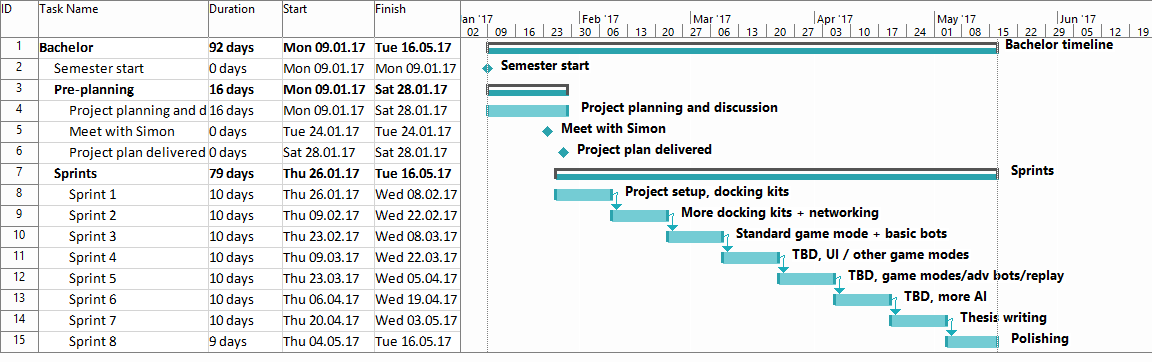
\includegraphics[width=1\textwidth]{images/gantt}
    \caption{Gantt chart from initial project plan}
    \label{fig:gantt}
\end{figure}

\subsection*{Milestones and Decisions}
We currently only have two major milestones in mind for the project. The first milestone is a working prototype of the game with a finished docking system. The second milestone is to have a working prototype with the standard game mode implemented. Due to the variable scope of the project it’s hard to estimate further milestones after this at this time.

All important design decisions and sprint meeting summaries will be documented in Confluence. The thesis itself will also be written directly in Confluence and later extracted to a PDF file. 

\subsection*{Time and resouce plan}
Time and resource planning will be done with the help of planning poker using story points, which will be done during the fortnightly sprint meetings, in accordance to our Scrum model. 
\chapter{Meeting Logs}
\section{Temporal record of meetings}
\subsection*{11.01.2016 - Bachelor Information Meeting}
Discussion of the process and setup of the thesis.  Deadlines for submission of documentation.  Introduction to the process and the sessions to help with writing the thesis.

\subsection*{24.01.2017}
Met with supervisor to discuss the project. Actions:
\begin{enumerate}
	\item Decide on a writing tool
	\item Install development environment
	\item Finish project plan
\end{enumerate}

\subsection*{30.01.2017}
First Sprint Planning Meeting for the project. Topics included:
\begin{description} 
    \item[Verify product backlog:]  The focus of the first sprint would be on project start up and docking kit architecture 
    \item[Primary issues of sprint: ] \mbox{}
    \begin{enumerate}
        \item Main Menu lobby containing join/leave functionality
        \item Docking kit architecture
        \item Marksman kit
    \end{enumerate}
\end{description}

\subsection*{09.02.2017}
Second Sprint meeting consisting of review, retrospective and planning:
\begin{itemize}
    \item What did we do well?
    \begin{itemize}
        \item Scoped well for the first sprint.
        \item Initial docking kit architecture is very robust
        \item Meeting up for daily scrum stand up
        \item Good use of Toggl
        \item Lobby seems to be fairly robust so far
    \end{itemize}
    
    \item What should we have done better?
    \begin{itemize}
        \item The start was a bit messy especially for Sondre and Martin as they struggled to parallellise the process of creating the first docking kit and architecture.
        \item Everyone could get a bit better at using smart commits more often and properly
    \end{itemize}
    
    \item Plan for next sprint:
    \begin{itemize}
        \item Primary focus on docking kits
        \item Bomber, Tank and Brawler kits
        \item Health management
        \item Status effects
    \end{itemize}
\end{itemize}

\subsection*{23.02.2017}
Third Sprint meeting consisting of review, retrospective and planning.

The scope for modifiers/status effects was a bit off so we had to spend a fair share of extra time to get it working properly. The Tank and Bomber kit were also unfinished by the end of the sprint so their completion has been put in the backlog for the next sprint.

\begin{itemize}
    \item What did we do well?
    \begin{itemize}
        \item Made a good and generic base architecture for our modifiers
    \end{itemize}
    
    \item What should we have done better?
    \begin{itemize}
        \item Remembering to set Jira issues to "in progress" once work has started.
        \item Sondre would have liked to start his work a bit earlier.
        \item Andreas got a bit stuck trying to restructure brawler abilities. Should have taken some extra time to properly get into the new modifiers architecture.
        \item Modifiers took longer to implement than expected
    \end{itemize}
    
    \item Plan for next sprint:
    \begin{itemize}
        \item Finish the docking kits (Tank and Bomber) that were left over from the previous sprint
        \item Trapper Kit.
    \end{itemize}
\end{itemize}

\subsection*{09.03.2017}
Fourth Sprint meeting consisting of review, retrospective and planning.

We got some decent progress during the previous sprint, but there are still some unfinished components for certain kits. We are kind of building the docking and ability architecture as we go. 
This is mainly because it is really hard for us to predict what we are going to need in the future. Working in a agile manner like this adds some additional overhead to the issues when working in several of the sprints. This sprint in particular required us to do a fair share of architectural work in order to provide abilities with the tools they needed to function as intended. 

\begin{itemize}
    \item Plan for the next sprint:
    \begin{itemize}
        \item Finish and polish all current kits as well as adding a few new ones to prepare for the implementation of the standard game mode.
        \item Sniper and Boomerang kits
        \item Revamp of the Marksman kit
        \item Getting familiar with ShareLaTeX
    \end{itemize}
\end{itemize}

\subsection*{10.03.2017}
Met with supervisor to discuss progress. Actions:
\begin{enumerate}
    \item Start thinking about thesis topics.
\end{enumerate}

\subsection*{23.03.2017}
Fifth Sprint meeting consisting of review, retrospective and planning.

The new kits developed during this sprint had pretty fun and interesting mechanics so we are fairly happy with their implementation. At this stage in development, the general workflow of creating docking kits has also been fairly solidified so efficiency slowly keeps increasing as we make more kits. We also performed a lot of code cleanup by trading virtual ability functions for interfaces which helps reduce boilerplate and improve code readability. 

In hindsight, we probably should have started to use interfaces earlier to make the code more clear and remove redundancy. There was still a bit of underscope this sprint as well for some kits, but not by much this time. 

The plan for the next sprint is to focus more on gameplay now that we have a decent amount of docking kits. We want to implement the standard game mode, in-game shop and start making sure that the various docking kits properly synchronise their behaviour based on teams rather than just local/non-local players. Since there are three of us on the group we decided to add another docking kit to the scope of this sprint so that everyone has something to work with as well. 

\subsection*{24.03.2017}
Met with supervisor to discuss progress. Actions:
\begin{enumerate}
    \item Transition more and more into thesis writing. Finish the most important functionality of the game that is required to be properly playable and write about the interesting challenges that we have encountered throughout the development of the game. 
\end{enumerate}

\subsection*{07.04.2017}
Sixth Sprint meeting consisting of review, retrospective and planning.

The shop functionality ended up being finished a bit earlier than expected. This allowed us to spend some extra time on writing the thesis, which can be thought of as a good thing.
We should probably have split up the standard game mode rather than thinking of it as a singular large task that would take multiple sprints to finish as it would reflect the progress better on Jira. 

The upcoming sprint takes place during Easter holidays so we don't expect too much progress taking place. What we would like to do is to move from Unity3D back to Unity2D as it cuts down a lot of data to synchronise across the network. We will end up saving one float for each Vector3 that we synchronise, which is a considerable amount. We believe that we are already close to hitting Unity's 4KB bandwidth limit so this is something we think might be worth spending some time to do. It might take some time to fix, but ultimately we think it might be worth it.
We would also like to take some time to write more in the thesis. 

\subsection*{20.04.2017}
Seventh Sprint meeting consisting of review, retrospective and planning. 

As expected, we did not get that much work done during the easter holidays. We did manage to get some writing done on the thesis, including a good draft for different topics to write about though. While moving to Unity2D might be good for the network performance of the game, the time spent porting the code might end up being better used on the thesis instead. 

The plan for the upcoming sprint is to primarily focus on writing the thesis and finishing up the last few components needed for the game to be complete. User testing will start taking place the moment the standard game mode is finished.
\chapter{Playtesting feedback and survey statistics}
\label{app:testFeedback}
This appendix includes the Google Form questions and answers for the playtesters and includes statistics for the different answers. One of the longer answers ended up not being printed fully due to limitations with Google Form and printing to PDF. 

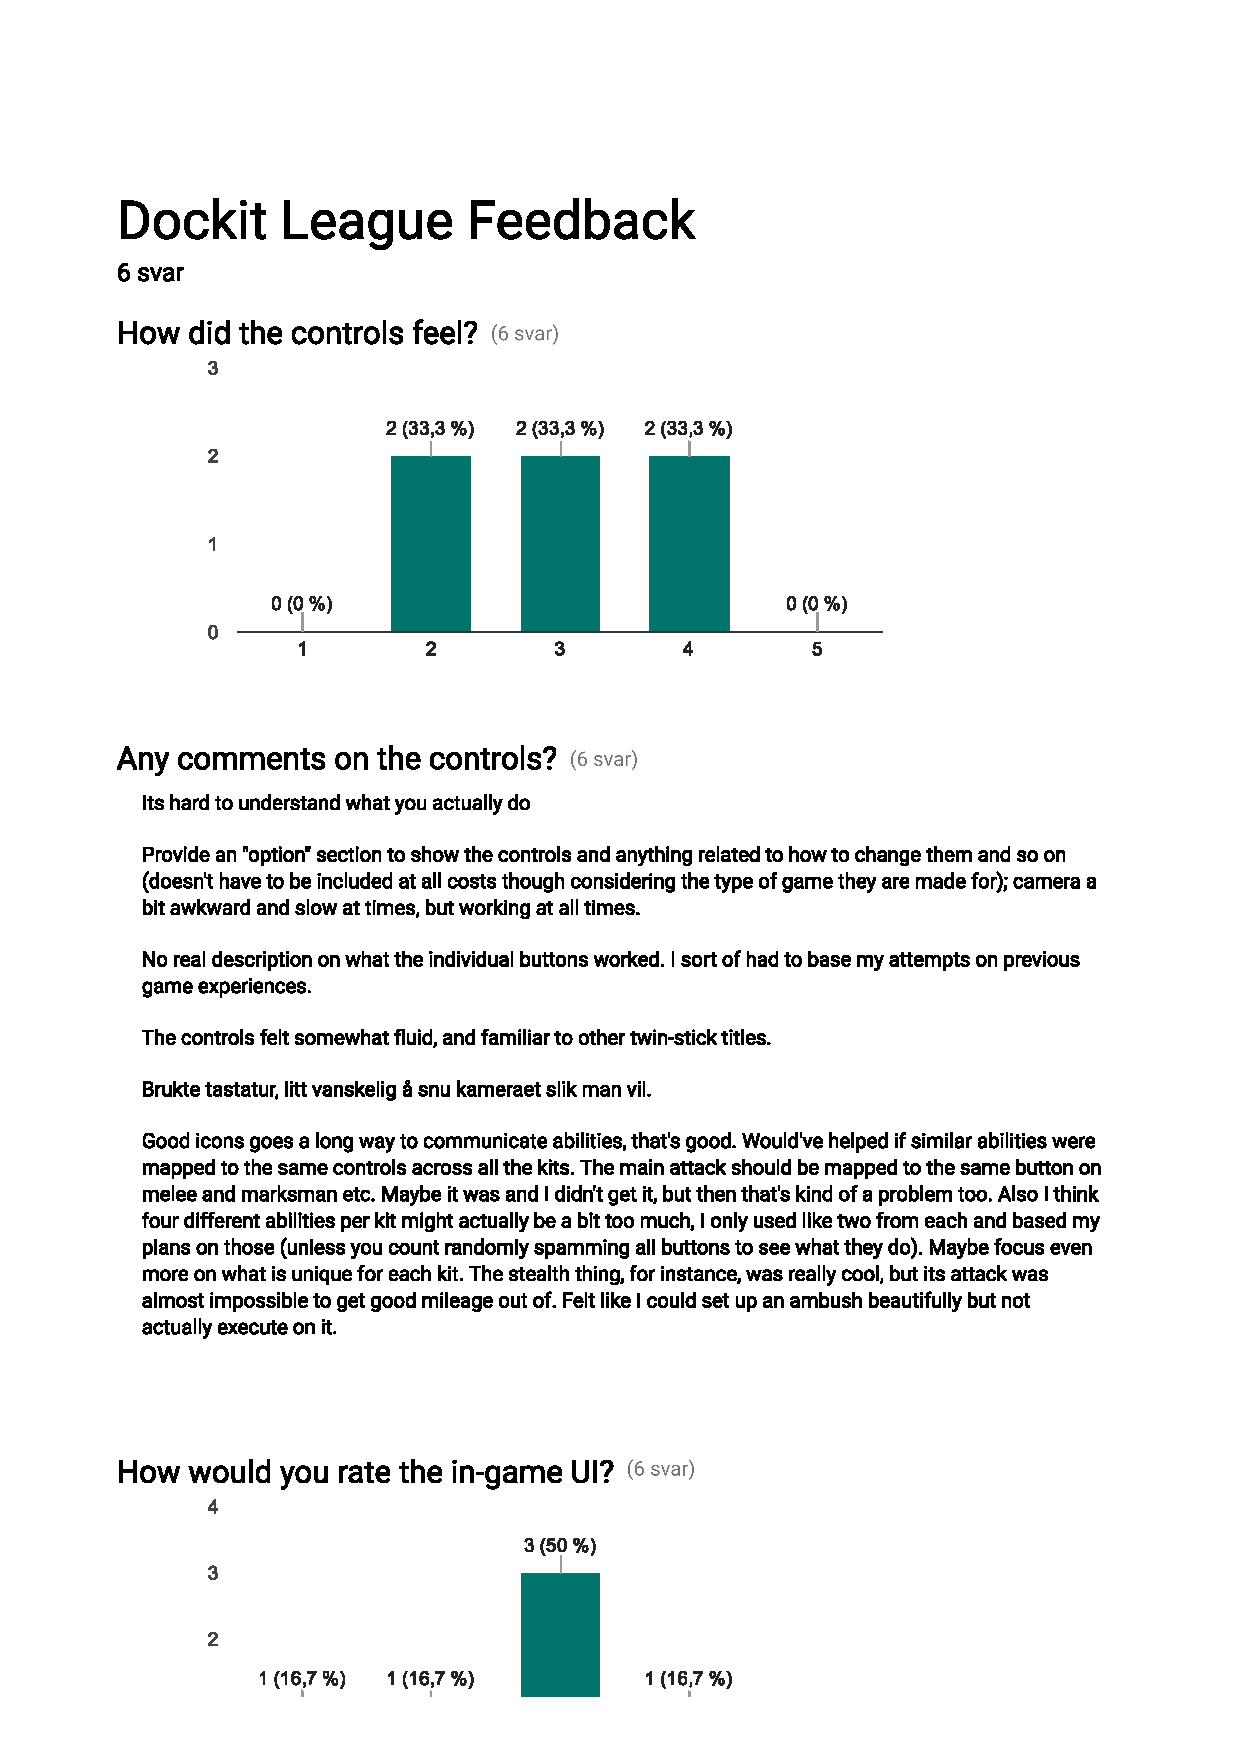
\includepdf[pages=-,pagecommand={}]{inc/DockitLeagueFeedback.pdf}
\chapter{Doxygen documentation}
This appendix includes a full doxygen documentation output from the project source code starting from the next page. 

%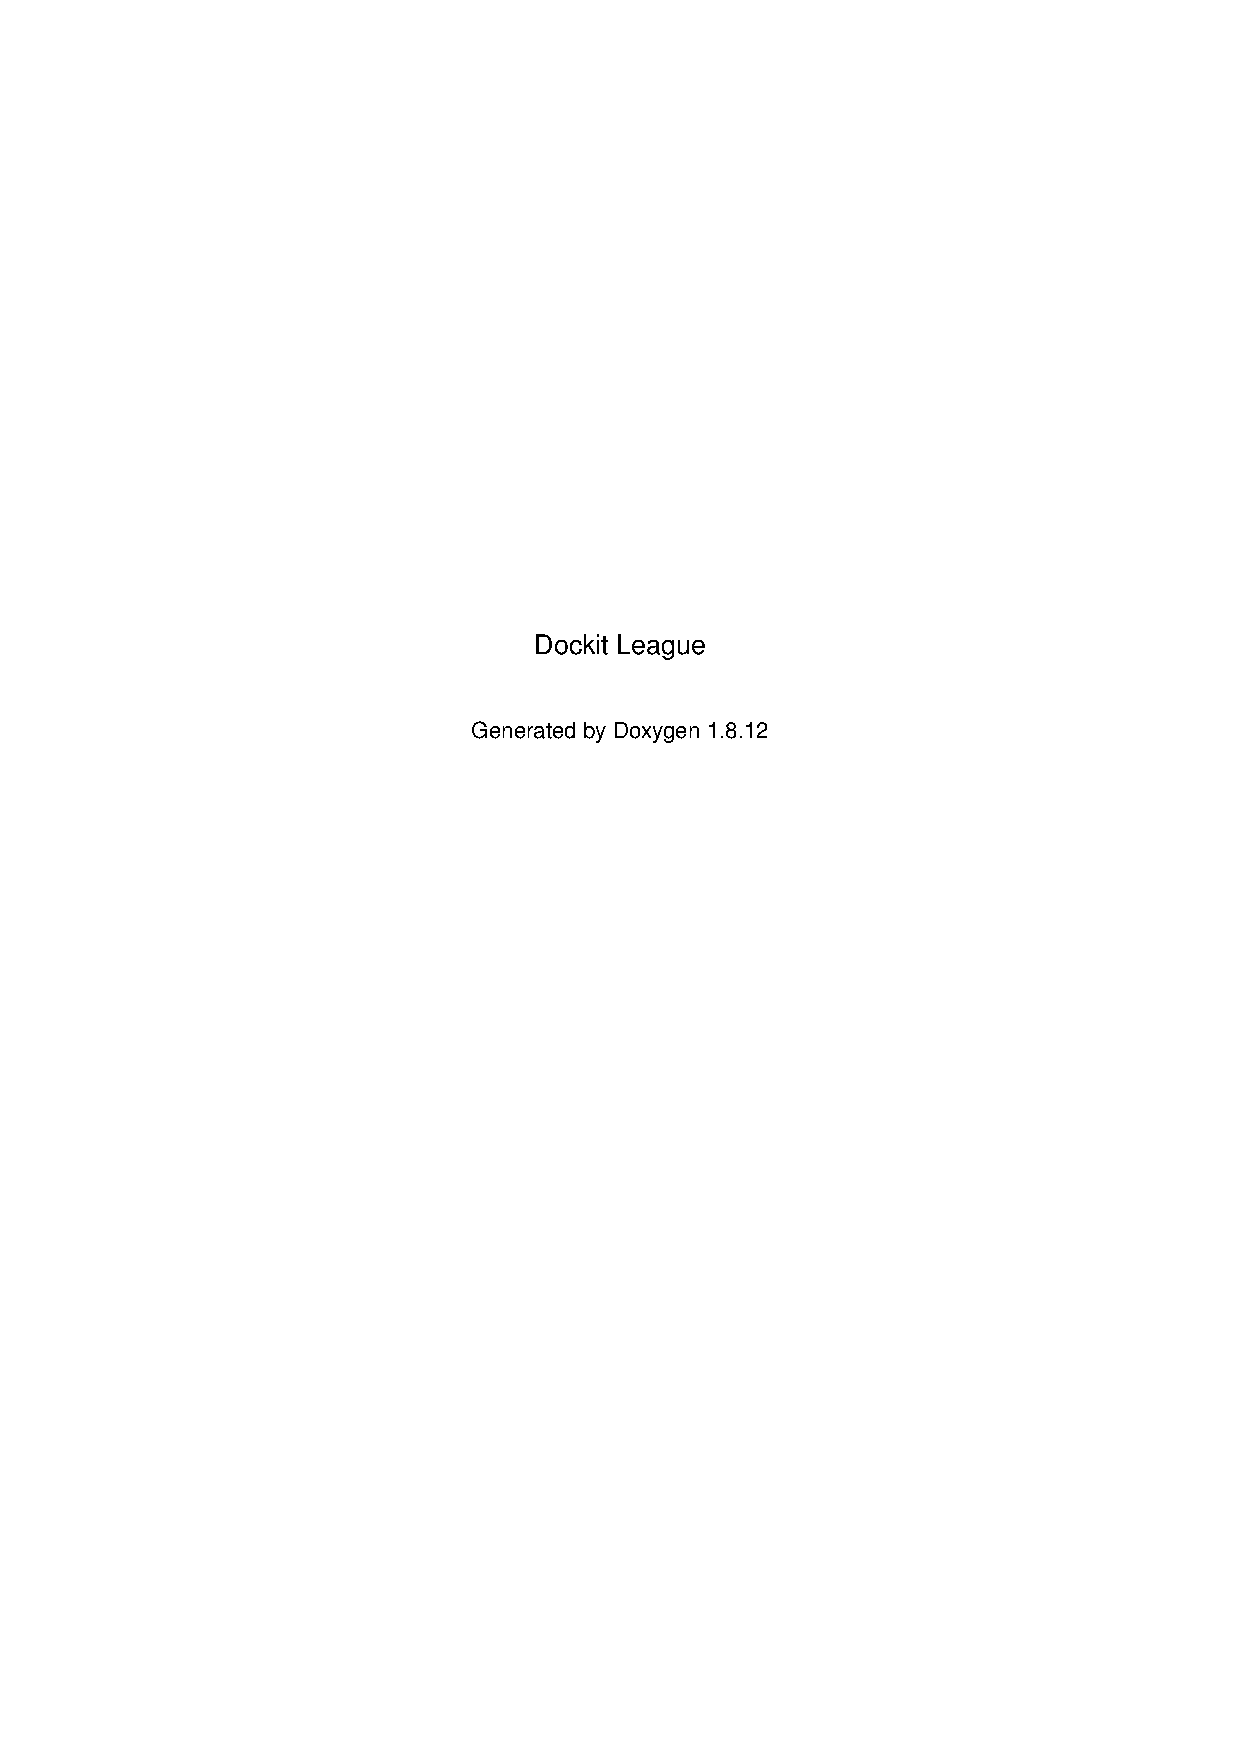
\includepdf[pages=-]{doxygenTest}

\end{document}
